\documentclass[preprint]{vldb}

\usepackage{amsmath,amssymb}
\usepackage{stmaryrd}
\usepackage{graphicx}
\usepackage{color}
\usepackage{trfrac}

\newcommand{\comment}[1]{}
\newcommand{\compiler}{DBToaster}
\newcommand{\tinysection}[1]{\noindent{\bf #1.}}
\newcommand{\tuple}[1]{{\langle#1\rangle}}
\newcommand{\todo}[1]{\textcolor{red}{#1}}
\newcommand{\note}[1]{\textcolor{blue}{#1}}



\begin{document}
\title{DBToaster: Lightweight Incremental Query Processing for Update-Intensive
Applications}
\numberofauthors{3}
\author{
\alignauthor
Yanif Ahmad\\
    \affaddr{Cornell University}
    \affaddr{Ithaca, NY}
    \email{yanif@cs.cornell.edu}
\alignauthor
Oliver Kennedy\\
    \affaddr{Cornell University}
    \affaddr{Ithaca, NY}
    \email{okennedy@cs.cornell.edu}
\alignauthor
Christoph Koch\\
    \affaddr{Cornell University}
    \affaddr{Ithaca, NY}
    \email{koch@cs.cornell.edu}
}
\maketitle

\begin{abstract}
Abstract goes here.
\end{abstract}


It is immediately plausible that one can do better than re-evaluate a query from scratch whenever the database changes a little. Incremental view maintenance (IVM) capitalizes on this insight \cite{DBLP:journals/tods/BunemanC79,DBLP:conf/sigmod/ShmueliI84,DBLP:conf/sigmod/BlakeleyLT86,roussopoulos-tods:91,DBLP:conf/vldb/CeriW91,DBLP:conf/deductive/GuptaKM92,DBLP:conf/sigmod/GuptaMS93,griffin-sigmod:95,yan-vldb:95,colby-sigmod:96,GHJ1996,kotidis-tods:01}. It is a solid, settled technique that has been implemented in many commercial DBMS, but has seen little new research activity in recent years and has gathered a little dust.

Now there is an exciting and potentially game-changing new development \cite{ahmad-vldb:09, koch-pods:10, kennedy-ahmad-koch-cidr:11}, an extreme form of IVM where all query evaluation work reduces to adding data (updates or materialized query results) to other materialized query results.  No join processing or anything semantically equivalent happens at any stage of processing. This works for a fragment of SQL with equijoins and aggregation, but without inequality joins or nesting aggregates.


Let us digest this, because the last claim goes counter to query processing intuitions to the point of absurdity. The main idea is the following: Classical IVM revolves around the idea that a materialized view can be maintained under updates by evaluating a so-called delta query and adding its result to the materialized view. The delta query captures how the query result changes in response to a change in the database. The new observation is that the delta query can be materialized and incrementally maintained using the same idea, making use of a delta query to the delta query, which again can be materialized and incrementally maintained, and so on, recursively. This works for classes of queries whose deltas are in some way structurally simpler than the base queries (e.g. having fewer joins), allowing this recursive query transformation to terminate. (It does so with a final trivial $k$-th delta query that does not refer to the database at all.) Termination is ensured for select-project-join queries with certain forms of aggregation, but some other features of SQL (specifically aggregations nested in where-conditions) have to be excluded. 

So where do the joins go? They {\em really} go away, as a benefit of incremental computation. If we want to compute $(x+1)*y$ and know $x*y$ and $y$, we only need to add $y$ to $x*y$, and the multiplication goes away. This is what happens when incrementally maintaining a join, where the join takes the place of multiplication. The pattern just sketched in basic algebra is not just an intuition but exactly what happens, and \cite{koch-pods:10} develops the algebraic framework to formalize this. We observe that the symbol 1 above represents the update workload.  In the incremental query processing framework, it must be a {\em constant} number of tuples that are changed in each incrementation step.

\comment{
To the reader who still cannot accept that joins can be replaced by no joins, we observe that the history of all incremental updates to the materialized view taken together is still essentially an execution of a nested loops join, that is, overall the value $x*y$ is constructed by adding $x$ copies of $y$. So if we put all the work associated with the individual updates happening over time together, the join work is still done. But refreshing the view in response to a single update does not require joins.
}

On paper, this approach clearly dominates classical IVM: if classical IVM is a good idea, then doing it recursively is an even better idea: The same efficiency-improvement argument for incremental maintenance of the base query also applies to the delta query. Argued from the viewpoint that joins are expensive and this approach eliminates them, one should expect a potential for excellent query performance.

But does this expectation translate into real performance gains? A priori, the cost of the bulk addition of materialized views or the costs associated with storing and managing additional auxiliary materialized views (for delta queries) might be more considerable than expected.


\medskip


This paper presents the lessons learned in an effort to realize recursive IVM, spanning nearly three years of intense work, to generalize it to be applicable on all or most of SQL, and to understand its strengths and drawbacks.
The contributions of this paper are as follows.
\begin{itemize}
\item
Multilevel IVM bears the promise of providing materialized views of complex SQL queries, without
window semantics or other restrictions, at very high refresh rates. We start by showing that there is
a need for such functionality, creating a benchmark consisting of automated trading and ETL workloads.
We show that state of the art systems cannot deliver materialized views refreshed at the rates
that some application domains (algorithmic trading, real-time analytics) require.
This is the challenge we set ourselves for the techniques and system described in this paper.

\item
We develop the vision of multilevel IVM further into a workable system.
While the techniques of \cite{ahmad-vldb:09, koch-pods:10} as well as existing implementations of
IVM in commercial DBMS are very restricted and exclude nested queries and other features of SQL,
we create the machinery to perform IVM and even recursive IVM on most of SQL (with the exception of
support for null values). To do this, we generalize the techniques of \cite{ahmad-vldb:09, koch-pods:10}
to not always materialize full delta queries but instead subexpressions that allow us to perform
IVM and maximize the performance obtained. This leads us to a query optimizer in which
the materialization of subqueries is a degree of freedom in optimization, and can be applied anywhere
in the input query or the delta queries obtained by applying this optimization.

To put ourselves in the position of using such an optimizer, we have to create suitable
intermediate representations of queries that support binding patterns for sideways information
passing, we study when and how to efficiently initialize views, and present query decomposition
and factorization techniques that lead to efficient formulations of update triggers that refresh our
views.

\item
Once high-level trigger programs for refreshing views based on multilevel IVM have been created,
we compile them further into highly efficient machine code.
We present our techniques for achieving this, which make use of sophisticated deforestation and
fusion techniques from the compilers literature.

\item
We have implemented our compiler and performed extensive experimentation with it. Our experiments
indicate that frequently, particularly for queries that consist of many joins of nested aggregation
subqueries that are not correlated through subqueries, our compilation approach dominates the
state of the art, often by multiple orders of magnitude. There are also queries in our benchmark
on which our techniques do not fare well; these usually involve the creation and maintenance of huge
auxiliary views whose data is rarely used by other views. These scenarios could be much improved upon
by suitable garbage collection strategies on auxiliary views. This is future work, and we consider
it likely that once such a technique has been integrated into our compiler, it will outperform the
state-of-the-art on an even wider range of queries.
\end{itemize}


The structure of the paper follows the order of contribution just laid out.















\comment{
This paper presents the lessons learned in an effort to realize aggressive IVM as motivated above. It represents an effort spanning nearly three years of intense work, which demonstrates that there are considerable technical challenges to be resolved. These key challenges are described next.


{\bf Compilation of update trigger code.}
%
The work that has to take place to update one materialized view with another (i.e., an auxiliary view representing a delta) is conceptually very simple; it essentially consists of bulk-adding tuple multiplicities of one view to another.

This updating work to be performed is particularly well-behaved and can be exploited for efficient evaluation:
\comment{
As observed in \cite{koch-pods:10}, this work is highly data-parallel. While parallel query evaluation is not the focus of the present paper, the updating work to be performed is particularly well-behaved. This can be exploited for efficient evaluation:
}
Classical query engines employ interpretation and large-gra\-nu\-la\-ri\-ty query operators such as joins to execute query plans.
In the past, IVM has used such query engines to evaluate its delta queries.
Instead, it is natural to avoid both query operators and plan interpretation, and the conceptual simplicity of the required work calls for aggressive code inlining and the elimination of the usual overheads due to interpreted query evaluation. It leads us to the compilation of view refreshing to lightweight machine code.

A considerable challenge is to determine suitable intermediate representations of query expressions to be used in the compiler. Such expressions in general have complex binding patterns which represent information flow. In general, this flow is not exclusively bottom-up.
Examples include complex conditions and nested subqueries correlated with their superqueries. Such expressions have input variables, and can only be evaluated if values for these input variables are given. In general, such expressions have to be materialized, which causes difficulties: how to determine a suitable domain for these input variables for which to materialize the results of the expressions, how to represent and store such materialized structures, and how to dynamically maintain the domains of input variables as updates add previously unseen values.


{\bf Compiler optimizations.}
%
Naively materializing delta queries, their delta queries, and so on causes the materialized views of the higher deltas to have high arity: in fact, the dimensionality can be as high as the arity of the product of all the relations joined together in the input query. The resulting size of the materialized views is of course unacceptable. As observed earlier \cite{ahmad-vldb:09, koch-pods:10} though, the materialized views can be losslessly decomposed into small views: taking a delta each time eliminates some join constraints, turning the views indeed into products.

This calls for factorization and decomposition techniques without which this approach would not be workable. In turn, however, recursive decomposition of delta queries of the various trigger programs (for insertions into and deletions from the relations occurring in the query) may produce large numbers of highly redundant factor views. This makes it essential to aggressively perform common subexpression elimination as well as deforestation and fusion techniques from the compiler literature.

In our implementation and experimentation efforts, this turned out to be much more important for satisfactory performance of the system than expected: without these techniques, recursive compilation for IVM with factorization as described in \cite{koch-pods:10} can result in hundreds of views to be maintained for a large join query, most of which are redundant and can be eliminated.
\comment{
Common subexpression elimination has been studied in the context of multi-query optimization, but here it takes a much more central role: without it, query performance will deteriorate by orders of magnitude almost every time: This is true even though we are referring to the compilation products of a single query, not a workload of multiple queries whose naturalness, if the queries share many subqueries, is often debatable. Thus, optimizations which are typically associated with compilers for general-purpose programming languages rather than query optimizers take a central role.
}
\comment{
We have also learned that some of the natural optimizations used in compilers for general-purpose programming languages rather than query optimizers take a central role. In particular, certain types of common subexpression elimination, loop fusion and analogous deforestation techniques for aggregations, are key to obtaining acceptable performance.
}
However, several of these optimizations such as deforestation have no form of expression in high-level query plan formalisms used in classical query optimization or recursive IVM. Thus, more than one internal intermediate representation (IR) of code is necessary.

\comment{
Our experiences led to two functional followed by one imperative IR. The functional IRs are a cleaned-up form of the algebraic expressions based on rings of queries and databases from \cite{koch-pods:10}, followed by a lower-level, Haskell-like and nearly general functional programming language in which we perform further forms of fusion and deforestation. The imperative IR is used in the compiler backend before imperative code generation. \comment{It is used for further optimizations that cannot be naturally expressed in a functional IR.} Overall, this leads us to a multi-stage reference compiler architecture for optimizing compilation of database queries to imperative code that we believe is general and relevant outside the context of incremental computation (cf. also Delite \cite{delite:11}).
}


\comment{
{\bf Side effects and initial value computation.}
%
Recursive IVM creates challenges we have not seen sufficient study of before, although they occur in simpler form in previous data management architectures that combine updating with querying, such as OLTP systems and stream processors: It is the tension between the convenience of viewing queries as pure functions of the data, and the {\em side-effects} that are updates.
In recursive IVM, an update triggers a variety of computations -- queries -- on various levels of a hierarchy of materialized views; one such computation creates data that is stored and used by another. These interleaved computations conceptually are meant to happen together, and side-effects must be carefully orchestrated to ensure a consistent database state after each update.

\comment{
In the context of recursive IVM, an update triggers a variety of computations -- queries -- on various levels of a hierarchy of materialized views; one such computation creates data that is stored and used by another. Compared to active databases, where certain events can trigger a cascade of computations, in the context of recursive IVM we face additional challenges in that interrelated computations do not profit from the benefits of isolation and conceptual serialization due to transaction semantics. The interleaved computations conceptually are meant to happen together.
}

As mentioned above, we in general need to materialize query expressions with binding patterns: queries that have input variables whose values cannot be determined from the query itself. The dynamic extension of the domains of these input variables and the resulting augmentation of the materialized views requires special initialization code distinct from the incrementation code (the compiled delta queries); this adds additional subtle challenges to the compilation framework. Most importantly, deciding how the domains of input variables of a materialized view has to be extended and optimizing the resulting code requires an intricate analysis of side effects across the hierarchy of materialized views.
} % end comment


{\bf Extraction/materialization as a first-class citizen of query optimizers.}
%
As stated above, the framework of recursive IVM requires delta queries to be structurally simpler than the queries they are deltas to. This is not the case for full SQL. This calls for abstracting from the strict notion of recursive IVM discussed in \cite{ahmad-vldb:09, koch-pods:10}. The key rewriting is to extract and materialize a subquery for IVM. This rewriting can be performed at multiple places in the query, as well as in delta queries that are used to incrementally maintain the materialization. In \cite{ahmad-vldb:09, koch-pods:10} the extracted subquery is always the full query or a factor in its product decomposition. But this is really an arbitrary restriction which can be lifted without causing fundamental problems.

This turns our compilation task into one of generating query evaluation code using an optimizer that has an {\em extract/materialize operator} that can be applied anywhere in the query, subject to optimization decisions (which we know from the literature on answering queries using views) but which also further compiles the delta queries auxiliary to materialization.


\medskip

The structure of the paper is as follows. Next, in Section~\ref{sec:sota}, we provide further motivation for the study of multilevel IVM by demonstrating by experimentation that low-latency continuous queries from ETL, monitoring and computational finance cannot be easily expressed by or managed by classical stream processors, or any other kind of existing engine. 
In Section~\ref{sec:compiler}, we present our compilation approach in detail, covering the various stages of a compiler from multilevel
incremental view maintenance to code generation.
Section~\ref{sec:experiments} returns to experimentation, picking up where we left off at the end of Section~\ref{sec:sota}, with all current data management systems failing to provide satisfactory performance for frequently fresh views for the workload proposed there.
We conclude with Section~\ref{sec:conclusion}.
} % end comment


\section{Incremental Queries}

\subsection{Map Calculus}

\def\calcsum{\mbox{Sum}}
\def\calceq{\mbox{{\tt =}}}
\def\calcgt{\mbox{{\tt >}}}
\def\calcgte{\mbox{{\tt >=}}}
\def\calclte{\mbox{{\tt <=}}}

\def \q{q}
\def \qq{Q}
\def \qqa{Q_1}
\def \qqb{Q_2}
\def \v#1{\mbox{#1}}
\def \vv#1{\mbox{{\tiny #1}}}

\begin{itemize}
  \item Overview of query language presentation: simple language exposing
  variables, that allows us to briefly present core transformations performed
  during compilation, followed by an extension to a more complex language that
  captures aspects of information flow and query evaluation.
\end{itemize}

\noindent Query language:

\begin{align*} 
\q \; \mbox{::-} &
  \;    c \;|\; Var(x)
  \;|\; R(\vec{x}) \;|\; m(\vec{x}) \;|\; f(\vec{x})
\\
\comment{
& \;|\; \theta(x,y)   \;|\; \theta_c(x)
  \;|\; \calceq(\q,y) \;|\; \calceq(x,y)
\\
}
\qq \; \mbox{::-} & \; \q \;|\; \calcsum(\vec{x}, \qq(\vec{x}\vec{y}))
    \;|\; \qqa(\vec{x}) + \qqb(\vec{y}) \;|\; \qqa(\vec{x}) * \qqb({\vec{y}}) \\
&   \;|\; -\qq(\vec{x}) \;|\; \theta(\qq) \;|\; \calceq(x,\qq)
\end{align*}

\begin{itemize}
  \item Basic terms ($q$) in language: constants, variables (i.e. variable
  usage), relations which define vars, maps which are keyed by vars, and
  functions which take vars as arguments.
  \item Higher-order terms ($Q$): sum aggregates with group-by vars
  listed (for presentation we drop this first arg if there are no group-bys), s
  sum and product operations of basic terms and higher-order terms. The
  variables listed for the subqueries are variables that are free in the
  subquery. \note{We return to free and bound variables in describing semantics
  below}. A sum operation corresponds to schema-less union, and a product to
  natural join. Note in the case of no variables from either $\qqa$ or $\qqb$
  these operations correspond to arithmetic sum and product. We also have
  additive inverse and nested queries, and a variable binding which associates
  (the value of) a variable to a subquery.
  \item Variable bindings are only introduced as part of our transformations,
  that is they are not needed to express SQL queries.
\end{itemize}

\noindent Language semantics:

\begin{align*}
c                   := & \; \tuple{} \mapsto c\\
Var(x)              := & \; \tuple{} \mapsto \Gamma(x)\\
R                   := & \; \vec{x} \mapsto R(\vec{x})\\
m                   := & \; \vec{x} \mapsto m(\vec{x}) \\
\comment{
\theta(x,y)         := & \; \tuple{x,y} \mapsto
                           \begin{cases}
                           1 \ldots x \; \theta \; y \\
                           0 \ldots \mbox{otherwise.}
                           \end{cases}\\
\theta_c(x)         := & \; \tuple{x} \mapsto
                           \begin{cases}
                           1 \ldots x \; \theta \; c \\
                           0 \ldots \mbox{otherwise.}
                           \end{cases}\\
\calceq(\q,y)       := & \; \tuple{y} \mapsto \q(\tuple{}) \\
\calceq(x,y)        := & \; \tuple{y} \mapsto \Gamma(x) \\
}
f                   := & \; \vec{x} \mapsto f(\vec{x}) \\
\end{align*}

\begin{align*}
\calcsum(\vec{x}, \qq(\vec{x}\vec{y})) := & \;
\vec{x} \mapsto \ \sum_{\vec{y}} \qq(\vec{x}\vec{y})
\\
\qqa(\vec{y}) + \qqb(\vec{z}) := & \;
\vec{x} \mapsto 
\sum_{\{\vec{x}\} = ext_{\vec{z}}(\vec{y}) \cup ext_{\vec{y}}(\vec{z})}
\qqa(\vec{x}) + \qqb(\vec{x})
\\
\qqa(\vec{y}) * \qqb(\vec{z}) := & \;
\vec{x} \mapsto \sum_{ \{\vec{x}\} = \{\vec{y}\} \Join \{\vec{z}\} }
\qqa(\vec{y}) * \qqb(\vec{z})
\\
-\qq(\vec{x}) := & \; \vec{x} \mapsto -\qq(\vec{x})
\\
\theta(\qq) := & \; \tuple{} \mapsto
                    \begin{cases}
                    1 \ldots \qq(\vec{x}) \theta 0\\
                    0 \ldots \mbox{otherwise.}
                    \end{cases}
\\
\calceq(x,\qq) := & \; \Gamma := \Gamma \cup \{x \mapsto \qq\};
                  \tuple{} \mapsto 1
\end{align*}

\begin{itemize}
  \item Based on generalized multiset relations (gmrs) of PODS paper, each
  expression in our language represents a finite function (ffn), whose
  arguments correspond to \textit{free} variables in the subquery. The domain
  of this finite function is the universe of named and typed tuples, the range
  the set of natural numbers, i.e. $f : \mbox{Tup} \mapsto \mathbb{N}$. Each
  finite function is non-zero for only a small subset of tuples.
  \item Semantics of basic terms:
  \begin{itemize}
    \item constants and variables are singleton functions, yielding the
    constant or variable value. Variables are bound in an environment,
    $\Gamma$, and for readability, we defer the full description of the bound
    and free variables in an expression to both later in this paper, and more
    formally in the PODS paper, especially with the definitions of safety in
    PODS Sec. 4, Fig. 1.
    \item Relations are ffns yielding cardinalities of tuples (i.e. multiset
    semantics), maps and functions yield values associated with keys (i.e.
    tuples), and arguments respectively.
  \end{itemize} 
  
  \item Semantics of higher-order terms:
  \begin{itemize}
    \item Sum aggregate is summation of (the values yielded by) an expression
    over non-group-by variables.
    \item Sum op is schema-less union, that is (the sum of counts of) all tuples
    from $\qqa$ and $\qqb$ extended to the combined schema of $\vec{y} \cup
    \vec{z}$. The $ext$ function performs this schema extension by ``adding''
    missing values. Note the semantics of missing values are not the same as
    nulls. In particular, our ffns are simply functions whose arguments must be
    \textit{consistent} with the values provided, that is variables whose
    values are missing can be ignored.
    \item Product op is (the product of counts of) tuples from $\qqa$ and
    $\qqb$ according to a natural join of said tuples.
    \item Additive inverse simply negates (the count of tuples in) a gmr.
    \item Nested aggregates are a singleton tuple (with count) based on a
    comparison of a subquery with no free variables (and thus a single-row
    subquery) to 0.
    \item Variable bindings add a mapping from the variable name $x$ to the
    ffn $\qq$ in the environment $\Gamma$, and yields an identity gmr. Note the
    ffn $\qq$ has no free variables.
  \end{itemize} 
  
\end{itemize}

\tinysection{Example queries}

\noindent VWAP:
\begin{verbatim}
select sum(price * vol)
from bids b0
where 0.25 * (select sum(b1.vol) from bids b1) >
     (select sum(b2.vol) from bids b2
      where b2.price > b0.price)
\end{verbatim}

\begin{align*}
\calcsum(\tuple{},
& B(\v{P0,V0}) * \v{P0} * \v{V0} *\\
& \calcgt(0.25 * \calcsum(B(\v{P1,V1}) * \v{V1}) \\
& \qquad \; \; - \calcsum(B(\v{P2,V2}) * \v{V2} * \calcgt(\v{P2-P0})))
\end{align*}

\comment{
\begin{align*}
\calcsum(\tuple{},
& B(P0,V0) * P0 * V0 *\\
& \calceq(\calcsum(B(P1,V1) * V1), X) * \\
& \calceq(\calcsum(B(P2,V2) * V2 * \calcgt(P2-P0)), Y) * \\
& \calcgt(0, 0.25 * X + Y)
\end{align*}
}

\noindent TPCH Q18:
\begin{verbatim}
select c.custkey, sum(l1.quantity)
from customer c, orders o, lineitem l1
where 1 <=
    (select sum(1) from lineitem l2
     where l1.orderkey = l2.orderkey
     and 100 < (select sum(l3.quantity)
                from lineitem l3
                where l2.orderkey = l3.orderkey))
and c.custkey = o.custkey
and o.orderkey = l1.orderkey
group by c.custkey;
\end{verbatim}

\begin{align*}
\calcsum(& \tuple{\v{CK}},
  \; C(\v{CK}) * O(\v{OK,OCK}) * L1(\v{OK1,Q1}) * \v{Q} * \\
& \; \calcgte(\calcsum(\tuple{}, L2(\v{OK2}) * 1 *
     \calceq(\v{OK1}+(-\v{OK2})) * \\
& \qquad \quad
    \calcgt(\calcsum(\tuple{}, L3(\v{OK3,Q3}) * \v{Q3} *
    \calceq(\v{OK2} - \v{OK3}))
\\ & \qquad \qquad + (-100)) + (-1)) * \\
& \; \calceq(\v{CK} - \v{OCK}) * \calceq(\v{OK} - \v{OK1})
\end{align*}

\subsection{Query Transformations}

\noindent This subsection presents core query transformations used for query
compilation, including:
\begin{itemize}
  \item Delta computation, the core query transformation needed for incremental
  processing. Compilation is essentialy computing higher-order deltas, i.e.
  recursively applying delta transformations, in conjunction with the other
  transformations below.
  \item Preaggregation, a transformation used to alter the structure of
  subqueries in expressions containing nested queries, to facilitate deltas of
  nested queries.
  \item Normalization and simplification, transformations used to bring a query
  to a canonical form, and reduce the query in terms of variables present.
\end{itemize}

\tinysection{Delta computation}
We define a function $\Delta$ that accepts a query, and a relation (and its
variables), for which to compute a delta query. This delta is identical to that
of the PODS paper (with the addition of a variable binding clause):
\begin{align*}
\Delta_{+R(\vec{x} \mapsto \vec{t})} c := & \; 0
\\
\Delta_{+R(\vec{x} \mapsto \vec{t})} Var(y) := & \; 0
\\
\Delta_{+R(\vec{x} \mapsto \vec{t})} R(\vec{x}) := & \;
\prod_i^{sch(\vec{x})} \calceq(t_i,x_i)
\\
\Delta_{+R(\vec{x} \mapsto \vec{t})} S(\vec{y}) := & \; 0
\\
\Delta_{+R(\vec{x} \mapsto \vec{t})}
\calcsum(\vec{x},\qq) := & \; \calcsum(\vec{x},\Delta\qq)
\\
\Delta_{+R(\vec{x} \mapsto \vec{t})} (\qqa + \qqb) := & \;
(\Delta\qqa + \Delta\qqb)
\\
\Delta_{+R(\vec{x} \mapsto \vec{t})} (\qqa * \qqb) := & \;
(\Delta \qqa * \qqb) +
(\qqa * \Delta \qqb) +
(\Delta \qqa * \Delta \qqb)
\\
\Delta_{+R(\vec{x} \mapsto \vec{t})} \theta(\qq) := & \;
(\theta(\qq + \Delta \qq) * \overline{\theta}(\qq)) \; -
\\
& \; (\overline{\theta}(\qq+\Delta \qq) * \theta(\qq))
\\
\Delta_{+R(\vec{x} \mapsto \vec{t})} \calceq(x,\qq) := & \;
    \calceq(x,\Delta \qq)
\end{align*}

\begin{itemize}
  \item Note every delta form, except deltas of nested queries, results in a
  simpler query in terms of the \textit{degree} of a query. Loosely speaking,
  a query's degree is a measure of the number of relations (and thus
  free variables) present in a query, and formally defined in PODS Sec. 5, Def.
  5.4.
  \item The delta for a nested query is not simpler, since we have both
  $\theta(\qq)$ and $\theta(\qq + \Delta \qq)$ present after applying the
  transformation. Given our query compilation algorithm is recursive in
  nature, query compilation has to intelligently determine how to compute
  higher-order deltas of nested queries to ensure termination.
\end{itemize}

\tinysection{Preaggregation}
Preaggregation is a transformation focusing on the complexity of queries
containing nested terms that essentially introduces additional aggregation
operations based on nesting structure and the correlated variables connecting
outer queries and nested queries.

\comment{
\begin{align*}
\calcsum(\phi[][\vec{x}] *
(\calcsum(\ldots)[\vec{x}][] * \calceq_\phi[y][] * (\psi[y][]))) \\
\end{align*}
}


\noindent The general form of a nested query is:
\begin{align*}
\calcsum(\vec{x}, \qqa * \theta(\qqb))
\end{align*}

\noindent where query $\qqb$ contains correlated variables, which are
free variables in $\qqa$. Preaggregation transforms query $\qqa$ to a group-by
aggregate, with the correlated variables in $\qqb$ as grouping variables.

\def \pa#1#2{\llbracket #1 \rrbracket_{PA}(#2)}

\noindent Preaggregation (note assumes left-associativity for product):

\begin{align*}
\pa{c}{\vec{x}} & := c
\\
\pa{Var(x)}{\vec{y}} & := Var(x)
\\
\pa{R(\vec{x})}{\vec{y}} & := \calcsum(\vec{x} \cap \vec{y}, R(\vec{x}))
\\
\pa{m(\vec{x})}{\vec{y}} & := \calcsum(\vec{x} \cap \vec{y}, m(\vec{x}))
\\
\pa{f(\vec{x})}{\vec{y}} & := \calcsum(\vec{x} \cap \vec{y}, f(\vec{x}))
\\
\pa{\calcsum(\vec{x}, \qq(\vec{x}\vec{y}))}{\vec{x}} & :=
    \calcsum(\vec{x}, \pa{\qq(\vec{x}\vec{y})}{\vec{x}})
\\
\pa{\qqa(\vec{y}) + \qqb(\vec{z})}{\vec{x}} & :=
    \pa{\qqa}{\vec{x}} + \pa{\qqb}{\vec{x}}
\\
\pa{\qqa(\vec{y}) * \qqb(\vec{z})}{\vec{x}} & :=
    \begin{cases}
    \calcsum(\vec{x}\vec{v}, 
        \pa{\qqa}{\vec{x}\vec{v}}) * \pa{\qqb}{\vec{x}} \\
    \; \; \ldots
        \mbox{ if $\vec{v} \neq \emptyset$},\vec{v} = \vec{y} \cap vars(\qqb)\\
    \pa{\qqa}{\vec{x}} * \pa{\qqb}{\vec{x}} \\
    \; \; \ldots \mbox{ otherwise}
    \end{cases}
\\
\pa{-\qq(\vec{y})}{\vec{x}} & := -\pa{\qq(\vec{y})}{\vec{x}}
\\
\pa{\theta(\qq)}{\vec{x}} & := \theta(\pa{\qq}{\tuple{})})
\\
\pa{\calceq(x,\qq)}{\vec{y}} & := \calceq(x, \pa{\qq}{\tuple{}})
\end{align*}

\noindent where $vars$ yields all variables used (that is $Var$ expressions)
in a query.

\noindent Preaggregation example:
\begin{align*}
\pa{\calcsum(\tuple{},
& B(\v{P0,V0}) * \v{P0} * \v{V0} *\\
& \calcgt(0.25 * \calcsum(B(\v{P1,V1}) * \v{V1}) \\
& \qquad \; \; - \calcsum(B(\v{P2,V2}) * \v{V2} * \calcgt(\v{P2-P0})))}
{\tuple{}} :=
\\[1ex]
\calcsum(\tuple{},
& \calcsum(\tuple{\v{P0}}, B(\v{P0,V0}) * \v{P0} * \v{V0}) *\\
& \calcgt(0.25 * \calcsum(B(\v{P1,V1}) * \v{V1}) \\
& \qquad \; \; - \calcsum(B(\v{P2,V2}) * \v{V2} * \calcgt(\v{P2-P0})))
\end{align*}

\begin{itemize}
  \item Apply preaggregation step. This ensures strictness of subqueries for
  correlated variables. Note preaggregation can be useful beyond nested
  queries, it essentially preaggregates relations to only those variables that
  are needed in the rest of the query. We return to this when describing our
  annotated calculus in the next section.
  \item Preaggregation results in a simpler substructure to the query (i.e.
  variables that are aggregated, are eliminated from the outer query).
  \todo{This definition of simpler is different than the concept of degree.
  Perhaps we can define this as the \textit{width} of a query, i.e. the number
  of outvars it has. Thus bigsum rewriting does not simplify in terms of
  degree, but does in term of width. With preaggregation, we are creating
  queries of minimal width w.r.t propagation.}
\end{itemize}

\tinysection{Query normalization and simplification}

\begin{itemize}
  \item Mostly refer to PODS paper.
\end{itemize}

\begin{itemize}
  \item Recursively monomial form
  \item Factorization
  \item Unifying loop variables
\end{itemize}



\subsection{Query Evaluation Annotations}

\begin{itemize}
  \item Input/output variables, cf. binding patterns, datalog.
  \item Provides a compact representation of the core data flow occuring during
        query evaluation, enabling a principled framework to perform all kinds
        of interesting optimizations.
  \item Annotated grammar, see below. Explain constraints on io-vars for
        base elements, e.g. relmaps. 
  \item Top down propagation, left to right propagation.
  \item Propagation diagram generic + for one of the annotated calculus
        examples.
  \item Determining input/output variables. Should occur as part of the
       compilation algorithm. \todo{Presentation: algorithm described before
       this, need to punt explanation of annotation to here.}
  \item \todo{Annotation rules for annotation algorithm?} 
\end{itemize}

\begin{align*} 
\q \; \mbox{::-} & \; R[][\vec{x}] \;|\; c[][] \;|\; Var[x][] \;|\;
m[\vec{x}][\vec{y}]\;|\; f[\vec{x}][]
\\
\comment{
& \;|\; \theta[x,y][] \;|\; \theta_c[x][] \;|\;
\calceq_\q[][y] \;|\; \calceq[x][y]
\\
}
\qq \; \mbox{::-} & \; \q[\vec{x}][\vec{y}] \;|\;
\calcsum(\q[\vec{x}][\vec{y}\vec{z}])[\vec{x}][\vec{z}] \\ & \;|\;
(\qqa[\vec{u}][\vec{v}] + \qqb[\vec{w}][\vec{x}])[\vec{y}][\vec{z}]
\\
& \;|\;
(\qqa[\vec{u}][\vec{vv'}] * \qqb[\vec{v'w}][\vec{x}])[\vec{y}][\vec{z}]
\\
& \;|\; \theta(\qq[\vec{x}][])[\vec{x}][]
\\
& \todo{\;|\; \calceq(\qq[\vec{x}][\vec{y}])}
\end{align*}

\begin{itemize}
\item Comment on lack of output vars in $\theta$, use of $y$ to
represent free var of bf-equality, which was previously an argument to
bf-equality

\item Propagation diagram:
    \begin{itemize}
      \item VWAP AST
      \item Transitive/multistep LR propagation
      \item Top-down bound var propagation, delta essentially binds a relation's
      variables from the very top
      \item No outvars on inequality constraints and nested queries, outvars only
      on bf-equalities
      \item Sum projection as explicit outvar restriction
    \end{itemize}

\end{itemize}

\noindent\todo{Punt annotated semantics to appendix/omit entirely. Should
explain two-level maps though.}

\begin{align*}
R[][\vec{x}]          := & \; \tuple{} \mapsto \vec{x} \mapsto R(\vec{x})\\
c[][]                 := & \; \tuple{} \mapsto \tuple{} \mapsto c\\
Var[x][]              := & \; \tuple{x} \mapsto \tuple{} \mapsto x\\
m[\vec{x}][\vec{y}]   := & \; \vec{x} \mapsto \vec{y} \mapsto
m(\vec{x})(\vec{y})
\\
\theta[x,y][]         := & \; \tuple{x,y} \mapsto \tuple{} \mapsto
                           \begin{cases}
                           1 \ldots x \; \theta \; y \\
                           0 \ldots \mbox{otherwise.}
                           \end{cases}\\
\theta_c[x][]         := & \; \tuple{x} \mapsto \tuple{} \mapsto
                           \begin{cases}
                           1 \ldots x \; \theta \; c \\
                           0 \ldots \mbox{otherwise.}
                           \end{cases}\\
\calceq_\q[][y]       := & \; \tuple{} \mapsto \tuple{y} \mapsto
                              \q(\tuple{})(\tuple{})
\\
\calceq[x][y]         := & \; \tuple{x} \mapsto \tuple{y} \mapsto x
\\
f[\vec{x}][\vec{y}]   := & \; \vec{x} \mapsto \vec{y} \mapsto f(\vec{x})
\\ 
\\
\calcsum(\q[\vec{x}] & [\vec{y}\vec{z}])[\vec{x}][\vec{y}] := \;
\vec{x} \mapsto \vec{y} \mapsto \ \sum_{\vec{z}} \q(\vec{x})(\vec{y}\vec{z})
\\
(\qqa[\vec{u}][\vec{v}] & + \qqb[\vec{w}][\vec{x}])[\vec{y}][\vec{z}] :=  \\
& \vec{y} \mapsto \sum_{ \{\vec{y}\} = \{\vec{u}\} \Join \{\vec{w}\} }
\vec{z} \mapsto  \sum_{ \{\vec{z}\} = \{\vec{v}\} \Join \{\vec{x}\} }
\qqa(\vec{u})(\vec{v}) + \qqb(\vec{w})(\vec{x})
\\
\\
(\qqa[\vec{u}][\vec{v_1}\vec{v_2}] & * \qqb[\vec{v_2}\vec{w}][\vec{x}])
[\vec{y}][\vec{z}] :=  \\
& \vec{y} \mapsto \sum_{ \{\vec{y}\} = \{\vec{u}\} \Join \{\vec{w}\} }
\vec{z} \mapsto \\
& \qquad \;\;\;
\sum_{ \{\vec{z}\} = \{\vec{v_1}\vec{v_2}\} \Join \{\vec{x}\} }
\qqa(\vec{u})(\vec{v_1}\vec{v_2}) * \qqb(\vec{v_2}\vec{w})(\vec{x}) 
\end{align*}


\tinysection{Annotated calculus examples}

\begin{itemize}
  \item TODO: what about io-vars inside new $\theta$ expression? Since
  $\theta$ inner expression must have no out-vars, how does the var propagation
  work for the inner expression?
\end{itemize}


%% VWAP with base io-vars
\begin{align*}
\calcsum( & B(\v{P0,V0})_{[][\vv{P0,V0}]} * \v{P0} * \v{V0} \; *
\\
& \calcgt(\calcsum(B(\v{P1,V1})_{[][\vv{P1,V1}]} * \v{V1})_{[][]} \; +
\\
& \quad \;\; \calcsum(B(\v{P2,V2})_{[][\vv{P2,V2}]} * \v{V2} *
                 \calcgt(\v{P2}-\v{P0})_{[\vv{P2,P0}][]})_{[\vv{P0}][]}
\\
& \quad )_{[\vv{P0}][]}
\\
& )_{[][]}
\end{align*}

%% VWAP with intermediate io-vars
\begin{align*}
\calcsum( & \tuple{},
    ((B(\v{P0,V0})_{[][\vv{P0,V0}]}
      * \v{P0})_{[][\vv{P0,V0}]}
      * \v{V0})_{[][\vv{P0,V0}]} *
\\
& \calcgt(\calcsum(\tuple{},
    (B(\v{P1,V1})_{[][\vv{P1,V1}]}
     * \v{V1})_{[][\vv{P1,V1}]})_{[][]} +
\\
& \quad \;\; \calcsum(\tuple{},
    ((B(\v{P2,V2})_{[][\vv{P2,V2}]} * \v{V2})_{[][\vv{P2,V2}]} *
\\
& \qquad \qquad
    \calcgt(\v{P2}-\v{P0})_{[\vv{P2,P0}][]})_{[][\vv{P2,V2}]})_{[\vv{P0}][]}
\\
& \quad )_{[\vv{P0}][]}
\\
& )_{[][]}
\end{align*}

%% Old example annotations, with bf-equalities
\comment{
\begin{align*}
\calcsum(((B[][P0,V0] * P0)[][] * V0)[][])
\end{align*}

\begin{align*}
\calcsum((B[][P0] * V0)[V0][])[V0][]
\end{align*}

\begin{align*}
\calcsum( & B[][P0,V0] * P0 * V0 *\\
& (\calcsum(B[][P1,V1] * V1)[][]) * \calceq[][X] * \\
& (\calcsum(B[][P2,V2] * V2 * >[P2,P0][])[P0][] * \calceq[][Y]) * \\
& ((((0.25 * X)[][] + Y)[][] * \calceq[][Z]) * 0[][] * >[Z][]))
\end{align*}


\begin{figure*}[htbp]
\begin{align*}
\calcsum( & ((B[][P0,V0] * P0)[][] * V0)[][] *\\
& ((\calcsum(B[][P1,V1] * V1)[][]) * \calceq[][X] * \\
& (\calcsum(B[][P2,V2] * Var[V2][] * >[P2,P0][])[P0][] * \calceq[][Y]))[][X,Y] *
\\ & ((((0.25 * X)[][] + Y)[][] * \calceq[][Z]) * >0[Z][])[][])[][]
\end{align*}
\end{figure*}
}

\noindent\todo{Punt/omit delta rules for annotated grammar}
%% Delta rules for annotated grammar
%%
\begin{align*}
\Delta_{+R(\vec{x} \mapsto \vec{t})} c[][] := & \; 0[][]
\\
\Delta_{+R(\vec{x} \mapsto \vec{t})} Var[y][] := & \; 0[][]
\\
\Delta_{+R(\vec{x} \mapsto \vec{t})} R[][\vec{x}] := & \;
\prod_i \calceq[t_i][x_i]
\\
\Delta_{+R(\vec{x} \mapsto \vec{t})} S[][\vec{y}] := & \; 0[][]
\\
\end{align*}

%% Old delta rules for agg,sum,prod w/ io-vars.
%% -- does not represent io-var changes to inner terms, making it useless
%%    for explaining changes to outer terms
\comment{
\begin{align*}
\Delta_{+R(\vec{t})}
\calcsum(\phi[\vec{w}][\vec{x}\vec{y}\vec{z}])[\vec{w}][\vec{x}\vec{y}]
:= & \;
\calcsum(\Delta\phi[\vec{w}][\vec{x}\vec{y}\vec{z}])
[\vec{t}\vec{w}][\vec{y}]
\\
\Delta_{+R(\vec{t})}
(\Phi[\vec{x}][\vec{y}] + \Psi[\vec{z}][\vec{w}])[\vec{u}][\vec{v}]
:= &
((\Delta\Phi[\vec{x}][\vec{y}]) + \Delta\Psi[\vec{z}][\vec{w}])
[\vec{t}\vec{u}][\ldots]
\\
\Delta_{+R(\vec{t})}
(\Phi[\vec{x}][\vec{y}] * \Psi[\vec{z}][\vec{w}])[\vec{u}][\vec{v}]
:= &
(((\Delta \Phi[\vec{x}][\vec{y}]) * \Psi[\vec{z}][\vec{w}])
[\vec{t}\vec{u}][\ldots] +
\\
& (\Phi[\vec{x}][\vec{y}] * \Delta \Psi[\vec{z}][\vec{w}])
[\vec{t}\vec{u}][\ldots] +
\\
& ((\Delta \Phi[\vec{x}][\vec{y}]) * \Delta \Psi[\vec{z}][\vec{w}])
[\vec{t}\vec{u}][\ldots])\\
& \; [\vec{t}\vec{u}][\vec{v}]
\\
\end{align*}
}

\noindent\todo{Rewrite as }

\[
\trfrac{
\Delta_{+R(\vec{x} \mapsto \vec{t})} \phi[\vec{uw}][\vec{xyz}] := 
\phi'[\vec{tw}][\vec{yz}]}
{
\begin{tralign}
\Delta_{+R(\vec{x} \mapsto \vec{t})}
\calcsum(\phi[\vec{uw}][\vec{xyz}])[\vec{uw}][\vec{xy}] & :=
     \calcsum(\Delta \phi[\vec{uw}][\vec{xyz}])[\ldots][\ldots] \\
& := \calcsum(\phi'[\vec{tw}][\vec{yz}])[\vec{tw}][\vec{yz}]
\end{tralign}
}
\]

\[
\trfrac{
\Delta(\Phi[\vec{ab}][\vec{cd}]) := \Phi'[\vec{ta}][\vec{c}] \qquad
\Delta(\Psi[\vec{wx}][\vec{yz}]) := \Psi'[\vec{tw}][\vec{y}]}
{
\begin{tralign}
\Delta((\Phi[\vec{ab}][\vec{cd}] + \Psi[\vec{wx}][\vec{yz}]) &
[\vec{abwx}][\vec{cdyz}]) := \\
& (\Phi'[\vec{ta}][\vec{c}] +
   \Psi'[\vec{tw}][\vec{y}])
  [\vec{taw}][\vec{cy}]
\end{tralign}
}
\]

\[
\trfrac{
\Delta(\Phi[\vec{ab}][\vec{cd}]) := \Phi'[\vec{ta}][\vec{c}] \quad
\Delta(\Psi[\vec{wx}][\vec{yz}]) := \Psi'[\vec{tw}][\vec{y}] \quad
\vec{cd} \cap \vec{wx} = \emptyset}
{
\begin{tralign}
\Delta((\Phi[\vec{ab}][\vec{cd}] * & \Psi[\vec{wx}][\vec{yz}])[abwx][cdyz])
:= \\
&    ((\Phi'[\vec{ta}][\vec{c}] *
       \Psi[\vec{wx}][\vec{yz}])[\vec{tawx}][\vec{cyz}] + \\
& \; (\Phi[\vec{ab}][\vec{cd}] *
       \Psi'[\vec{tw}][\vec{y}])[\vec{tabw}][\vec{cdy}] + \\
& \; (\Phi'[\vec{ta}][\vec{c}] *
      \Psi'[\vec{tw}][\vec{y}])[\vec{taw}][\vec{cy}])[\vec{tabwx}][\vec{cdyz}]
\end{tralign}
}
\]

\noindent\todo{Finish below -- add intermediate io-vars to product case.}

\noindent\todo{Is this case correct? Why should we care about propagated
variables w.r.t to deltas? Can a delta violate propagation and safety?}
\[
\trfrac{
\Delta(\Phi[\vec{ab}][\vec{cdm}]) := \Phi'[\vec{ta}][\vec{c}] \qquad
\Delta(\Psi[\vec{mwx}][\vec{yz}]) := \Psi'[\vec{tw}][\vec{y}]}
{
\begin{tralign}
\Delta((\Phi[\vec{ab}][\vec{cdm}] * \Psi[\vec{mwx}][\vec{yz}])[][])
:= & \;
     ((\Phi'[\vec{ta}][\vec{c}] *
       \Psi[\vec{wx}][\vec{yz}])[][] + \\
& \; (\Phi[\vec{ab}][\vec{cd}] *
       \Psi'[\vec{tw}][\vec{y}])[][] + \\
& \; (\Phi'[\vec{ta}][\vec{c}] *
      \Psi'[\vec{tw}][\vec{y}])[][])[][]
\end{tralign}
}
\]


\[
\trfrac{
\Delta_{+R(\vec{t})}(\Phi[\vec{ab}][]) := \Phi[\vec{ta}][]
}
{
\begin{tralign}
\Delta_{+R(\vec{t})} \theta(\Phi[\vec{ab}][])[\vec{ab}][]
:= & \;
( \theta(\Phi[\vec{ab}][] + \Delta \Phi[\vec{ta}][])[\vec{tab}][] * \\
& \; \;
\overline{\theta}(\Phi[\vec{ab}][])[\vec{ab}][] -
\\
& \; \; \overline{\theta}(\Phi[\vec{ab}][] + \Delta \Phi[\vec{ta}][])
[\vec{tab}][] *
\\
& \; \; \theta(\Phi[\vec{ab}][])[\vec{ab}][]
)[\vec{tab}][]
\end{tralign}
}
\]

\section{Query Compilation}

\def\algsum{\mathrm{sum}}
\def\algagg{\mathrm{agg}}
\def\algtop{\mathrm{top}}
\def\algtopk{\mathrm{topk}}

\def\algsumr{\mbox{sumr}}
\def\algsumf{\mbox{sumf}}
\def\distinct{\mbox{distinct}}
\def\routerjoin{\bowtie\!=}

We now present \compiler's compilation algorithm through an example
illustrating how queries are turned into efficient procedural code. Our
compilation framework applies to the core relational algebra and group-by
aggregates, and uses a custom query algebra to define map data structures. These
maps are closely related to views definable by SQL aggregate group-by queries but
at the same time are main memory data structures that are easy to access in
applications. Due to space limitations we only present the small fraction
of our map algebra transformations used to derive code for our example query.

\noindent\textbf{Compilation example.} Consider the query below on three
relations and schemas $R(A,B), S(B,C), T(C,D)$:

\begin{verbatim}
select sum(A*D) from R, S, T
where R.B=S.B and S.C=T.C
\end{verbatim}

Next, given the data and query model above, relations $R, S, T$ are
manipulated via update streams which consist of the standard requests
of inserting, updating and deleting tuples. For ease of presentation, we can
consider updates as pairs of delete and insert requests. We start with handling
an insert to the relation $R$, with a tuple $\{\tuple{a,b}\}$. Assuming
the variable $q$ maintains the query result, we can show:

\smallskip
Insert R(a,b):
\begin{eqnarray*}
\Delta q &=& \algsum_{A*D}(\{\tuple{a,b}\} \bowtie S \bowtie T)
\\ &=&
\algsum_{A*D}(\{a\} \times \sigma_{B=b}(S) \bowtie T)
\\ &=&
\algsum_{a*D}(\sigma_{B=b}(S) \bowtie T)
\\ &=&
a * \underbrace{\algsum_{D}(\sigma_{B=b}(S) \bowtie T)}_{q_D[b]}
\end{eqnarray*}

Above $q_D[b]$ is an example of a map that we use to compute the change in query
result $q$, a map with key-value pair entries of keys $b$, and values defined as
the result of the query: $\algsum_{D}(\sigma_{B=b}(S) \bowtie T)$. While we do
not go into the full details of the derivation validity, we can see it is a
simplification of the original query by considering the relation $R$ as a
singleton relation $\{\tuple{a,b}\}$. We can symmetrically derive for inserting
into relation $T$ as: $\Delta q = d * q_A[c]$, resulting in a map
$q_A[c] = \algsum_{A}(R \bowtie \sigma_{C=c}(S))$. The insertion to $S$ is:

\smallskip
Insert S(b,c):
\begin{eqnarray*}
\Delta s &=& \algsum_{A*D}(R \bowtie \{\tuple{b,c}\} \bowtie T)
\\ &=&
\algsum_{A*D}(\sigma_{B=b}(R) \times \sigma_{C=c}(T))
\\ &=&
\underbrace{\algsum_{A}(\sigma_{B=b}(R))}_{q_A[b]} *
\underbrace{\algsum_{D}(\sigma_{C=c}(T))}_{q_D[c]}
\end{eqnarray*}



\begin{figure*}[tb]
\begin{center}
\begin{tabular}{|l|l|l|l|l|l|}
\hline
Recursion level & Event & Query $q$ & Code for $\Delta q$ & Maps & Map
definition\\
\hline
1 & $+R$ & $\algsum_{A*D}(R \bowtie S \bowtie T)$
& $a*q_D[b]$ & $q_D[b]$ & $\algsum_{D}(\sigma_{B=b}(S) \bowtie T)$
\\
\hline
1 & $+S$ & $\algsum_{A*D}(R \bowtie S \bowtie T)$
& $q_A[b] * q_D[c]$ & $q_A[b]$ & $\algsum_{A}(\sigma_{B=b}(R))$
\\
& & & & $q_D[c]$ & $\algsum_{D}(\sigma_{C=c}(T))$
\\
\hline
1 & $+T$ & $\algsum_{A*D}(R \bowtie S \bowtie T)$
& $d*q_A[c]$ & $q_A[c]$ & $\algsum_{A}(R \bowtie \sigma_{C=c}(S))$
\\
\hline
2 & $+R$ & $\algsum_{A}(R \bowtie \sigma_{C=c}(S))$
& $\mbox{foreach($c$): } a * q_1[b,c]$ & $q_1[b,c]$ &
$\algsum_{1}(\sigma_{BC=bc}(S))$
\\
2 & $+R$ & $\algsum_{A}(\sigma_{B=b}(R))$
& $a$ & & \\
\hline
2 & $+S$ & $\algsum_{A}(R \bowtie \sigma_{C=c}(S))$
& $q_A[b]$ & & 
\\
2 & $+S$ & $\algsum_{D}(\sigma_{B=b}(S) \bowtie T)$
& $q_D[c] $ & & 
\\
\hline
2 & $+T$ & $\algsum_{D}(\sigma_{B=b}(S)\bowtie T)$
& $\mbox{foreach($b$): }d * q_1[b,c]$ & $q_1[b,c]$ &
$\algsum_{1}(\sigma_{BC=bc}(S))$
\\
2 & $+T$ & $\algsum_{D}(\sigma_{B=b}(T))$
& $d$ & & \\
\hline
3 & $+S$ & $\algsum_{1}(\sigma_{BC=bc}(S))$
& $1$ & & \\
\hline
\end{tabular}
\end{center}
\label{tab:derivation}
\caption{\compiler's recursive compilation of the query:
\texttt{select sum(a*d) from R, S, T}, showing the query being compiled, the
procedural code required to incrementally compute the query result, maps
required by the code, and the query defining the map.}
\end{figure*}


Note the elimination of any join in the above query since we are able to exploit
distributivity properties of summation and multiplication, and the cross product
operator. At this point we have presented one level of compilation, for an
insertion into each base relation $R, S, T$, resulting in incremental query
result computation code, a set of maps which we have to maintain, and queries
defining the map contents. At this point, we recursively compile the map
definition queries, considering each of the three types of insertion (to
$R,S,T$), and subsequently aggressively inline any code generated into a handler
for each type of insertion. For example, consider the maps $q_A[c], q_A[b]$
above, whose entries are dependent on the relation $R$. We recursively compile
incremental maintenance of this map for insertions to $R$ as:

\smallskip
Insert R(a,b):
\begin{eqnarray*}
\Delta q_A[b] &=& \algsum_{A}(\{\tuple{a,b}\}) = a
\\
\mbox{foreach $c$: }
\Delta q_A[c] &=& \algsum_{A}(\{\tuple{a,b}\} \bowtie \sigma_{C=c}(S))
\\ &=&
\algsum_{a}(\sigma_{BC=bc}(S))
\\ &=&
a * \underbrace{\algsum_{1}(\sigma_{BC=bc}(S))}_{q_1[b,c]}
\end{eqnarray*}

Above, we use $\algsum_{1}$ to refer to a count aggregate, that is 
$\algsum_{1}(\sigma_{BC=bc}(S))$ is a count of $\tuple{b,c}$ tuples in S.
Note the \textit{foreach} statement when computing $\Delta q_A[c]$. This arises
since a single tuple $\tuple{a,b}$ in $R$ affects all map entries with keys
$c^*$ where the relation $S$ contains tuples $\tuple{b,c^*}$. Again our
compilation is symmetric for the relations $R$ and $T$ due to the nature of the
join graph in this query. Thus the maintenance code for maps $q_D[b], q_D[c]$
is:

\smallskip
Insert T(c,d):
\begin{eqnarray*}
\Delta q_D[c] &=& d\\
\Delta q_D[b] &=& \mbox{foreach(c): } d * q_1[b,c]
\end{eqnarray*}

\noindent For an insertion to $S$, we must maintain maps $q_A[c], q_D[b]$:

\smallskip
Insert S(b,c):
\begin{eqnarray*}
\Delta q_A[c] &=&
\algsum_{A}(R \bowtie \{\tuple{b,c}\})
\\ &=&
\algsum_{A}(\sigma_{B=b}(R) \times \{c\})
\\ &=&
\algsum_{A}(\sigma_{B=b}(R))
\;=:\; q_A[b]
\\
\Delta q_D[b] &=&
\algsum_{D}(\{\tuple{b,c}\} \bowtie T)
\\ &=&
\algsum_{D}(\{b\} \times \sigma_{C=c}(T))
\\ &=&
\algsum_{D}(\sigma_{C=c}(T))
\;=:\; q_D[c]
\end{eqnarray*}

\noindent Note that we are already maintaining maps $q_A[b], q_D[c]$ above, that
is there are opportunities for sharing maps across event handler functions.
Finally, we can maintain $q_1[b,c]$ following insertions to $S$ simply as:
$\Delta q_1[b,c] = 1$.
For thoroughness, we show the resulting handler functions from this example,
following the inlining of each code fragment generated at each recursive step
below.

\begin{verbatim}
on insert into R values (a,b) {
   s += a * s_D[b];   s_A[b] += a;
   foreach c (in Cs[b]) do
      s_A[c] += a * s_1[b,c];
}

on insert into S values (b,c) {
   s += s_A[b] * s_D[c];   s_A[c] += s_A[b];
   s_D[b] += s_D[c];       s_1[b,c] += 1;
}

on insert into T values (c,d) {
   s += s_A[c] * d;   s_D[c] += d;
   foreach b (in Bs[c]) do
      s_D[b] += s_1[b,c] * d;
}
\end{verbatim}

Additionally Table~\ref{tab:derivation} compactly describes this compilation
example, including the case of deletion events which turn out to be strictly analogous in
this case due to the fact that sum aggregates have a well defined inverse in the
subtraction operator.


\comment{
Query compilation in \compiler\ is founded on an algebra for manipulating a map
data structure. Our map algebra is related to SQL queries through the use of a
map to represent a group-by aggregate. A map algebra expression, or map for
short, is defined as one of the following forms:
\[
f_1 + f_2
\quad\;\;
f_1 * f_2
\quad\;\;
c
\quad\;\;
x
\quad\;\;
\algsumf_f(Q)
\]
where $f, f_1, f_2$ are map algebra expressions, $c$ are numerical constants,
$x$ are variables, and $Q$ are positive relational algebra
expressions.

Variables in maps are {\em free} unless they are {\em bound}. Given a map $f$
with free variables $\vec{x}$ (enumerated in the order in which they first appear
in $f$), $f[\vec{a}]$, where $\vec{a}$ is a tuple of variables and constants of
the same arity as $\vec{x}$ denotes each $x_i$ in $f$ substituted by $a_i$. The
variables $\vec{x}$ in $f[\vec{a}]$ are then called bound. So, for instance, the
free variables of $5 * x + y$ are $x,y$ and $(5 * x + y)[z, 2]$ is $5 * z + 2$
with free variable $z$. The number of free variables in a map is also called the
map's dimension.

(Positive) relational algebra expressions are built using relation names,
selection $\sigma$, projection $\pi$, relational product $\times$, union $\cup$,
constant singleton relations $\{\vec{a}\}$,
and renaming $\rho$.
Column names $A$ are treated like bound variables.
Selection conditions are comparisons
$f \;\theta\; 0$ where $\theta \in \{ =, \neq, <, \le, >, \ge \}$.
Projections may compute additional columns
using map algebra expressions, i.e.\ the syntax is
$\pi_{\vec{A}, f_1 \rightarrow B_1, \dots, f_k \rightarrow B_k}(Q)$. 

We use a multiset semantics for relations as in SQL; none of the operations
of relational algebra eliminate duplicates.
Otherwise, the semantics of relational algebra expressions $Q$ is standard.
Variables in $\vec{x}$ are {\em bound}\/ to constants from above; thus, 
the semantics of an aggregate map $\algsumf_f(Q)$ without free variables
is a single numerical value $v$ such that
\[
\algsumr_A(\pi_{f \rightarrow A}(Q))[] = \{ \tuple{v} \}.
\]
where $\algsumr$ is the ungrouped sum aggregate of SQL.

\subsection{Map compilation}
The goal of this section is to provide an algorithm for compiling map algebra
expressions into efficient C code that incrementally maintains the
maps they define.
We will need the following general-to-specific ordering $\prec$ on maps.


\begin{definition}\em
A map $f$ is called (strictly) {\em more specific than}\/ a map $f'$,
denoted $f \prec f'$, if $f$ can be obtained from $f'$ by replacing
one or more relation names occurring in $f'$ by fixed singleton relations.
\end{definition}


Note that this replacement may occur deep inside a map, not just in the topmost
relational algebra subexpression. For example,
\[
\algsumf_A(\pi_{\algsumf_B(\rho_B(\tuple{b})) + 2}(S))
\prec
\algsumf_A(\pi_{\algsumf_B(\rho_B(R)) + 2}(S))
\]


\begin{figure*}[t!]
%\begin{algorithm}
\begin{eqnarray*}
\Delta_{+R(\vec{r})} c       &:=& 0 \\
\Delta_{+R(\vec{r})} x       &:=& 0 \\
\Delta_{+R(\vec{r})} (f + g) &:=&  (\Delta_{+R(\vec{r})} f) + (\Delta_{+R(\vec{r})} g) \\
\Delta_{+R(\vec{r})} (f * g) &:=& f * (\Delta_{+R(\vec{r})} g) 
                              +   (\Delta_{+R(\vec{r})} f) * g                        
                              +   (\Delta_{+R(\vec{r})} f) * (\Delta_{+R(\vec{r})} g)
\\
\Delta_{+R(\vec{r})} \algsumf_A(\{ \vec{a} \}) &:=& 0
\\
\Delta_{+R(\vec{r})} \algsumf_{A_i}(\rho_{\vec{A}}(R)) &:=& r_i
\\
\Delta_{+R(\vec{r})} \algsumf_A(S) &:=& 0
\\
\Delta_{+R(\vec{r})}  \algsumf_A(Q_1 \cup Q_2) &:=&
\Delta_{+R(\vec{r})} (\algsumf_A(Q_1) + \algsumf_A(Q_2))
\\
\Delta_{+R(\vec{r})} \algsumf_{f[\vec{A};\dots] * g[\vec{B};\dots]}(\rho_{\vec{A}}(Q_1) \times \rho_{\vec{B}}(Q_2)) \; &:=&
\Delta_{+R(\vec{r})} \big( \algsumf_{f[\vec{A};\dots]}(\rho_{\vec{A}}(Q_1))
    * \algsumf_{f[\vec{B};\dots]}(\rho_{\vec{B}}(Q_2)) \big)
\\
\Delta_{+R(\vec{r})} \algsumf_A(\pi_{f + g \rightarrow A}(Q)) &:=&
\Delta_{+R(\vec{r})} \big( \algsumf_A(\pi_{f \rightarrow A}(Q))
   + \algsumf_A(\pi_{g \rightarrow A}(Q)) \big)
\\
\Delta_{+R(\vec{r})} \algsumf_A(\pi_{f[\vec{x}] \rightarrow A}(Q)) &:=&
   (f + \Delta_{+R(\vec{r})} f)
   * \Delta_{+R(\vec{r})} \algsumf_1(Q)
\\
\Delta_{+R(\vec{r})} \algsumf_A(\pi_{f \rightarrow A}(Q)) &:=&
   \algsumf_A(\pi_{\Delta_{+R(\vec{r})} f \rightarrow A}(Q)) \\
   &+& \algsumf_A(\pi_{f \rightarrow A}(\Delta_{+R(\vec{r})} Q)) \\
   &+& \algsumf_A(\pi_{\Delta_{+R(\vec{r})} f \rightarrow A}(\Delta_{+R(\vec{r})} Q))
\\
\Delta_{+R(\vec{r})} \algsumf_A(\sigma_{g \theta 0}(Q)) &:=&
\mbox{if ($\Delta_{+R(\vec{r})} g \;\theta\; 0$) then
   $\algsumf_A(Q + \Delta_{+R(\vec{r})}(Q))$} \\
&& \mbox{else if ($(g + \Delta_{+R(\vec{r})} g \;\theta\; 0) \Rightarrow
(g \;\theta\; 0)$) then $- \algsumf_A(Q)$ else 0}
\end{eqnarray*}
%\end{algorithm}
%
\caption{Recursive algorithm for compiling the
on insert into $R$ values $\vec{r}$ trigger.}
\label{fig:mainalg}
\end{figure*}


Figure~\ref{fig:mainalg} shows our compilation algorithm for maps, the core
procedure of the DBToaster compiler. Given a map $f$, it inductively computes a
delta-expression that does not use relational algebra.

It is easy to verify that the right-hand sides of the rewriting are successively
simpler by either being dominated by the left-hand sides under the general-to-specific
ordering $\prec$ or being sums or products of
strictly shorter expressions.

Thus, the output of the rewriting algorithm given a map is a delta map that does not
contain aggregates or relational algebra. However, the rewriting may add new free
variables, i.e., starting from a map $f[\vec{x}]$, we may obtain an aggregate-free
map $g[\vec{x}, \vec{y}]$. We then {\em marginalize}\/ over these as follows,
\[
\Delta f[\vec{x}] = \sum_{\vec{y}} g(\vec{x}, \vec{y}). 
\]

Rather than explaining the rules in full detail here, we simply note that these
rules can be thought of as being similar to pattern matching, where the right
hand side map can be used to replace any matching left hand side. Furthermore,
note that the chain of derivations directly represent the code we must generate
and execute in our tuple-processing functions.

\subsection{Compilation Example}
We briefly provide an example application of our map rewrites on the following
aggregate query:

\[
s := \algsum_{A*D}(R \bowtie S \bowtie T).
\]

For illustration we simply consider the insertion of a new tuple into
solely the relation R. Also, since this example is only meant to be a brief
illustration due to space restrictions, we omit the case for deletions.

\begin{itemize}
\item
Insert R(a,b):
\begin{eqnarray*}
\Delta s &=& \algsum_{A*D}(\{\tuple{a,b}\} \bowtie S \bowtie T)
\\ &=&
\algsum_{A*D}(\{a\} \times \sigma_{B=b}(S) \bowtie T)
\\ &=&
\algsum_{a*D}(\sigma_{B=b}(S) \bowtie T)
\\ &=&
a * \underbrace{\algsum_{D}(\sigma_{B=b}(S) \bowtie T)}_{s_D[b]}
\end{eqnarray*}

\end{itemize}

 
Next, we incrementally maintain $s_D[b]$, which in this case is maintained by
insertions into S.

\begin{itemize}
\item
Insert S(b,c):
\begin{eqnarray*}
\Delta s_D[b] &=&
\algsum_{D}(\{\tuple{b,c}\} \bowtie T)
\\ &=&
\algsum_{D}(\{b\} \times \sigma_{C=c}(T))
\\ &=&
\algsum_{D}(\sigma_{C=c}(T))
\;=:\; s_D[c]
\end{eqnarray*}
\end{itemize}

Thus the code is:
\begin{verbatim}
on insert into R values (a,b)
{
   s += a * s_D[b];

   // Updates from R to other maps...
}

on insert into S values (b,c)
{
   s += s_A[b] * s_D[c];
   s_D[b] += s_D[c];
   // Updates from S to other maps...
}

// code for T ...
\end{verbatim}
}

\section{Query Evaluation}

\subsection{Structural Recursion}

\def\ktclist{\mbox{List}}
\def\ktcmap{\mbox{Map}}
\def\apply{\mbox{apply}}
\def\seq{\mbox{seq}}
\def\ifelse{\mbox{ifelse}}
\def\mem{\mbox{mem}}
\def\lookup{\mbox{lookup}}
\def\slice{\mbox{slice}}
\def\setval{\mbox{set\_value}}
\def\setmap{\mbox{set\_map}}
\def\ktmap{\mbox{map}}
\def\ktflat{\mbox{flatten}}
\def\ktagg{\mbox{agg}}
\def\ktgb{\mbox{gb\_agg}}
\def\ktpwl{\mbox{pairwith}_1}
\def\ktpwr{\mbox{pairwith}_2}
\def\ktext{\mbox{ext}}
\def\ktid{\mbox{id}}

\begin{align*}
e \; \mbox{::-} & \; c \;|\; v \;|\; e + e \;|\; e * e \;|\; e \; \theta \; e
\;|\; e \neq 0?\; e : 0 \\
& |\; \mem(t,\vec{e}) \;|\; \lookup(t,\vec{e})\\
t \; \mbox{::-} & \; \ktclist(t) \;|\; \ktcmap(id,\vec{v_i},\vec{v_o})
  \; | \; \slice(t,\vec{e}) \;|\; \tuple{\vec{e}} \;|\; \pi_{\vec{i}}(t) \\
& |\; \lambda v . t \;|\; \Lambda v1,v2.t \;|\; \apply(t,t)
  |\; \seq(\vec{t}) \;|\; \ifelse(e,t,t) \\
& |\; \ktmap(t,t) \;|\; \ktflat(t) \;|\; \ktagg(t,e,t) \;|\; \ktgb(t,e,t,t)\\
& |\; \setval(id,\vec{e},\vec{e},t) \;|\; \setmap(id,\vec{e},t)
\end{align*}

\begin{itemize}
  \item Notational extensions for transformations, i.e. representations of
  composition and pairwith. Lets us write things in the same way as the Kleisli
  paper.
\end{itemize}

\begin{align*}
f \circ g & := \lambda x. \apply(f, \apply(g,x))
\\
f \times g & := \lambda xy. \tuple{apply(f, x), apply(g, y)}
\\
f \circ (g \times h) & := \lambda xy.
\apply(f, \tuple{\apply(g, x), \apply(h, y)})
\\
\ktext(f,x) & := \ktflat(\ktmap(f,x))
\\
\ktpwl(x,y) & := \lambda \tuple{x,y}. \ktmap(\lambda z.\tuple{z,y}, x)
\\
\ktpwr(x,y) & := \lambda \tuple{x,y}. \ktmap(\lambda z.\tuple{x,z}, y)
\end{align*}

\def \sr#1{\llbracket #1 \rrbracket_{SR}}

\tinysection{Map accesses}
\begin{itemize}
  \item Conditionals to test map key existence, potentially resulting in
  intial value computation.
  \item Updates to persistent collections for IVC.
  \item Map accesses yielding internal slice representation, i.e. collections.
  Statement RHS evaluation applies operations to whole collection, i.e.
  iteration/scans over the entire data structure rather than doing any
  complicated lookups/random accesses, suggesting a simple list-based
  implementation.
\end{itemize}

\begin{align*}
\sr{m[ & \vec{x}][\vec{y}] \tuple{init}} := \; \apply(\\
  & \lambda it. \ifelse(\mem(it, \vec{x}), \\
  & \quad \apply(\\
  & \quad \quad
    \lambda ot. \ifelse(\mem(ot, \vec{y}), \psi(ot, \vec{y}),\\
  & \quad \quad \quad
    \apply(\lambda iv. \seq(\phi(ot,\tuple{},\vec{y},iv), iv), \sr{init})), \\
  & \quad \quad \lookup(it, \vec{x})), \\
  & \quad \apply(\lambda iv.
       \seq(\phi(it,\vec{x},\vec{y},iv), iv), \sr{init})),\\
  & \ktcmap(m,\vec{x},\vec{y}))\\
\mbox{where} & \; \psi(m,\vec{x}) := 
                        \begin{cases}
                        \lookup(m,\vec{x}) & \mbox{if bound($\vec{x}$)}\\
                        \slice(m,\vec{x})  & \mbox{otherwise}
                        \end{cases}\\
\mbox{and}   & \; \phi(m,\vec{x},\vec{y},v) :=
                        \begin{cases}
                        \setval(m, \vec{x}, \vec{y}, v) & \mbox{if is\_val($v$)}
                        \\
                        \setmap(m, \vec{x}, v) & \mbox{otherwise}
                        \end{cases}
\end{align*}

\noindent\todo{Define bound(), is\_val() above}

\tinysection{Products, conditionals and bigsums}

\begin{align*}
\sr{e_1[\vec{w}][\vec{x}] \; & \theta \; e_2[\vec{y}][\vec{z}]} :=
  \ktflat(
\\
  \ktmap( & \lambda \vec{x}v_1.
  \ktmap(\lambda \vec{z}v_2. \tuple{\vec{x}\vec{z},\theta(v1,v2)},
         \sr{e_2[\vec{y}][\vec{z}]}),
\\
& \sr{e_1[\vec{w}][\vec{x}]}))
\\
\sr{e_1[\vec{x}][] \neq 0 \; ? \; & e_2[\vec{y}][\vec{z}] : 0} :=
\\
&
\begin{cases}
\sr{e_1[\vec{x}][]} \neq 0 \; ? \; \sr{e_2[\vec{y}][]} : 0
& \mbox{if $\vec{z} = \tuple{}$}
\\
e_2[\vec{y}][\vec{z}] * (e_1[\vec{x}][] \neq 0 \; ? \; 1 : 0)
& \mbox{otherwise}
\end{cases}
\end{align*}

\noindent\todo{Rewrite product in Kleisli form, i.e. with prod+prep phases}

\noindent\todo{Aggregation function semantics, i.e. what are x,y?}
\begin{align*}
\sr{ & m[\vec{x}][\vec{y}] \; \mbox{{\tt +}=} \sum_{\vec{z}}
    e[\vec{x}][\vec{y}\vec{z}]} :=
\\
& \begin{cases}
  \ktagg(\Lambda v_1,v_2. v_1+v_2 , 0,
         \sr{e[\vec{x}][\vec{y}\vec{z}]})
  & \mbox{if $\vec{y} = \tuple{}$}
  \\
  \ktgb(\Lambda v_1,v_2. v_1+v+2 , 0, \lambda \vec{y}\vec{z}.\vec{y},
        \sr{e[\vec{x}][\vec{y}\vec{z}]})
  & \mbox{otherwise}
  \end{cases}
\\
\sr{ & m[\vec{x}][\vec{y}] \; \mbox{:=} \sum_{\vec{z}}
    e[\vec{x}][\vec{y}\vec{z}]} :=
\\
& \begin{cases}
  \ktagg(\Lambda v_1,v_2. v_1+v_2 , 0, \sr{e[\vec{x}][\vec{y}\vec{z}]})
  & \mbox{if $\vec{y} = \tuple{}$}
  \\
  \ktgb(\Lambda v_1,v_2. v_1+v_2 , 0, \lambda \vec{y}\vec{z}.\vec{y},
        \sr{e[\vec{x}][\vec{y}\vec{z}]})
  & \mbox{otherwise}
  \end{cases}
\\
\end{align*}

\begin{itemize}
  \item Products as structural recursion composed map.
  \item LHS$\rightarrow$RHS projection+aggregation as structural recursion
  group-by aggregate.
  \item Bigsums as structural recursion aggregate.
\end{itemize}

\tinysection{External functions}
\begin{itemize}
  \item Several external functions required, which we cannot optimize in terms
  of structural recursion. However it turns out these all occur following
  statement RHS evaluation for maintaining the LHS map. These external
  functions are:
  \item Slice merging, i.e. combining delta and existing slice
  \item In var tier iteration. Allows us to avoid having side-effecting
  iteration as part of our language fragment, that is every expression in our
  language fragment yields a collection (which of course may be a singleton).
\end{itemize}

\tinysection{Structural recursion example}
\begin{itemize}
  \item Translation of VWAP M3 example to structural recursion.
  \begin{itemize}
    \item \todo{Awkward to write out map access code in full.}
    \item \todo{The goal should be to really represent the maps and aggregates
    applied to slice accesses for products etc in VWAP.}
  \end{itemize}
\end{itemize}

\def \srin#1{\llbracket #1 \rrbracket_{\mbox{\tiny{In}}}}
\def \srsub#1#2{(#1)[#2]}

\subsection{Program Optimization}
\begin{itemize}
  \item Product optimizations, define in monadic form, i.e. w/ type judgements
  in our grammar. 
  \begin{itemize}
    \item Define binary product/join in Kleisli syntax, and composition of
    binary joins, i.e. with maps as scans, and pairwith/prep composers,
    \item Show how this representation can capture any join tree, i.e.
    l/r-deep, bushy, etc.
    \item Discuss intermediates from composing, i.e. same as modern query plans.   
    \item Show transformation to a single n-way representation w/ no
    intermediates, listing inlining and substitution rules for Kleisli to our
    representation.
    \item Discuss need for optimizer, and how no current system optimizes both
    the arity of the join operator in addition to the composition plan. Our
    representation here lays the groundwork for this.
  \end{itemize}
  \item Aggregation pushdown, also w/ type judgements, using our grammar.
  \item Lookup lifting and combined delta+initial value optimization.
  \item Optimization examples.
  \item Category theory morphisms diagrams for optimizations.
\end{itemize}

\begin{align*}
\srin{\lambda \tuple{x,y}. & \apply(f \circ \ktpwl, \tuple{x,y})} :=
\\
    & \lambda \tuple{x,y}. \apply(f[2 \mapsto y], x)
\\
\srin{\lambda \tuple{x,y}. & \apply(f \circ \ktpwr, \tuple{x,y})} :=
\\
    & \lambda \tuple{x,y}. \apply(f[1 \mapsto x], y)
\\
\srin{\apply( & \lambda x.f, y)} := f[1 \mapsto y]
\\
\srin{\apply( & \lambda \tuple{x_1 \ldots x_n}.f, \tuple{y_1 \ldots y_n})} :=
\\
    & f[1 \mapsto y_1, \ldots, n \mapsto y_n]
\\
\srin{\apply(& f \circ g, y)} := \apply(f, g[1 \mapsto y])
\\
\srin{\apply(& f \circ g, \tuple{y_1,\ldots,y_n})} :=
\\
    & \apply(f, g[1 \mapsto y_1,\ldots,n \mapsto y_n])
\\
\srin{\lambda xy. \apply( & f \circ (\ktid \times h), xy)} :=
\\
    & \lambda xy. \apply(f, \tuple{x, \apply(h, y)})
\\
\end{align*}

\begin{align*}
\srsub{\lambda \tuple{x,y}. \apply(f, \tuple{x,y})}{1 \mapsto c} & :=
    \lambda y. \apply(f, \tuple{c,y})
\\
\srsub{\lambda x. \apply(f \circ g, x)}{1 \mapsto c} & :=
    \apply(f, g[1 \mapsto c])
\\
\srsub{\lambda c. \ktmap(\lambda \tuple{x,y}.
    \apply(f, \tuple{x,y}), c)}{1 \mapsto a} & :=
\\
    \lambda c. \ktmap( & \lambda y. \apply(f, \tuple{a,y}), c)
\end{align*}

\noindent\todo{Think about substitution more.
\begin{itemize}
  \item Substitution is not clean, requires lineage, i.e. subst of first
  argument is ambiguous for maps. We might want to subst both the map function,
  and the map function arg w.r.t tuples
\end{itemize}}

\noindent Aggregation transformation:

\begin{align*}
\ktagg(\Lambda_f, i) \circ \ktflat =
    \ktagg(\Lambda_f, i) \circ \ktmap(\ktagg(\Lambda_f, 0))
\end{align*}

\tinysection{Discussion}
\todo{Discussion of why such an approach can't be applied to standard
  relational plans? They can, query plan optimization has traditionally been
  applied to operators, whose design in turn has been focused on efficient
  out-of-core execution. Imperative and functional language compilers and
  optimizers have focused much more aggressively on a variety of optimization
  techniques for in-memory applications and our backend begins to touch on how
  to bridge this gap. e.g., how do we do schema/tuple-layout based register
  allocation}

\newcommand{\figurewidth}[0]{1.8in}

\newcommand{\tablefig}[1]{
  \hspace*{-0.25in}
  \includegraphics[width=\figurewidth]{../graphs/graphs/#1}
}

\begin{figure}
\begin{center}
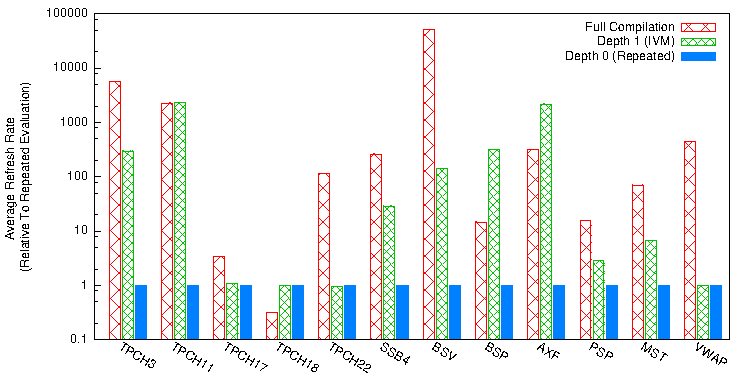
\includegraphics[width=3.4in]{../graphs/graphs/bakeoff.pdf}
\caption{Cross-query comparison of our compiler in different depth-restricted modes, and the best performing streaming and database engine for each query.  Note the logscale on the y-axis.}
\label{fig:experiments:bakeoff}
\end{center}
\end{figure}

\begin{figure*}
\begin{center}

\begin{minipage}{\textwidth}
\begin{center}
\hspace*{0.1in}
\begin{tabular}{cccc}
\tablefig{unified_tpch3.pdf} &
\tablefig{unified_tpch11.pdf} &
\tablefig{unified_tpch17.pdf} &
\tablefig{unified_ssb4.pdf} \\
(a) & (b) & (c) & (d)
\end{tabular}
\caption{TPC-H Query 3~(a), 11~(b), 17~(c), and SSB4~(d): (a) By the 40\%\ marker, all streams except LINEITEM have completed, and the remaining tuples consume no additional memory. (b) For simple two-way joins, full compilation is virtually identical to depth 1. (c) Due to the nested aggregate, IVC requires a nested loop, while full compilation requires only a single scan.(d) Full compilation is a full polynomial order faster than in IVC, although performance does begin to drop once the system begins running out of memory around the 27\%\ marker.}
\label{fig:experiments:tpch3}  
\label{fig:experiments:ssb4}
\label{fig:experiments:tpch17}
\label{fig:experiments:tpch11}
\end{center}
\end{minipage}

\vspace*{0.2in}

\begin{minipage}{\textwidth}
\hspace*{0.1in}
\begin{tabular}{cccc}
\tablefig{unified_brokervariance.pdf} & 
\tablefig{unified_tpch22.pdf} &
\tablefig{unified_vwap.pdf} &
\tablefig{unified_serverload.pdf} \\
(a) & (b) & (c) & (d)
\end{tabular}
\caption{BSV~(a), TPC-H Query 22~(b), VWAP~(c), and SVL~(d):  (a) The many-to-many relationship on the join term forces IVM to perform linear work on each insertion, which full compilation avoids.  (b) The small CUSTOMER stream completes at the 10\%\ marker, while the remaining ORDERS tuples require only linear time with full compilation. (c) IVM repeatedly re-evaluates the nested (parameterized) sub-query, while full compilation maintais a cache of sub-query results. (d) Materializing nested queries gains a polynomial degree of performance over IVM, but memory continues to grow. }
\label{fig:experiments:brokervariance}
\label{fig:experiments:tpch22}
\label{fig:experiments:vwap}
\label{fig:experiments:serverload}
\end{minipage}

\vspace*{0.2in}

\begin{minipage}{\textwidth}
\hspace*{0.1in}
\begin{tabular}{cccc}
\tablefig{unified_pricespread.pdf} &
\tablefig{unified_missedtrades.pdf} &
\tablefig{unified_axfinder.pdf} &
\tablefig{unified_brokerspread.pdf} \\
(a) & (b) & (c) & (d)
\end{tabular}
\caption{PS~(a), MST~(b), AXF~(c) and BSP~(d):  (a,b) The performance and memory plateaus result from a portion of the trace from about 0.001\%\ to 0.01\%, where a single order is repeatedly placed and revoked. (c,d) Full compilation's aggressive materialization strategy results in the caches growing too large to be efficiently maintained.}
\label{fig:experiments:pricespread}
\label{fig:experiments:MST}
\label{fig:experiments:axfinder}
\label{fig:experiments:brokerspread}
\end{minipage}



\end{center}
\end{figure*}

\begin{figure*}
\begin{center}

%\begin{minipage}{\textwidth}
%\begin{center}
%\begin{tabular}{ccc}
%(a) & (b) & (c)
%\end{tabular}
%\caption{TPC-H Query 18~(a). }
%\label{fig:experiments:tpch18}
%\end{center}
%\end{minipage}
%
\vspace*{0.1in}

\begin{minipage}{\textwidth}
\begin{center}
\begin{tabular}{cccc}
\tablefig{unified_tpch18.pdf} &
\tablefig{unified_5gig_tpch3.pdf} &
\tablefig{unified_5gig_tpch11.pdf} &
\tablefig{unified_5gig_tpch22.pdf} \\
(a) & (b) & (c) & (d)
\end{tabular}
\caption{TPCH Query 18 (a): An incorrectly chosen join ordering prevents full compilation from effectively exploiting foreign key dependencies in the TPC-H schema;  The three fastest-running TPC-H queries (3~(b), 11~(c), and 22~(d)) run on a 5GB dataset: (b) Quadratic effects from early parts of the workload become apparent in IVM at this scale, while full compilation remains linear. (c) Maintaining the base relations already projected and aggregated gives a slight edge to full compilation at this scale.  (d) Full compilation performance is reduced due to updates being linear in the size of CUSTOMER, but still performs better than depth 1.}
\label{fig:experiments:big}
\label{fig:experiments:big:tpch3}
\label{fig:experiments:big:tpch11}
\label{fig:experiments:big:tpch22}
\end{center}
\end{minipage}

\end{center}
\end{figure*}

We now analyze the performance of our compilation techniques.  As in Section \ref{sec:dbfail}, our experiments are run on Redhat Enterprise Linux running in a VM with 16 GB of RAM, and 2x4 core Intel Xeon E5620 2.4 GHz processors allocated to it.  Note that our compiler produces single-threaded code, while other platforms were allowed to consume the full resources of the VM.

Our analysis uses the same queries and methodology as in Section~\ref{sec:tscomparison}: The queries are described in Section~\ref{sec:tscomparison:workload}, and expressed in SQL form in Appendix~\ref{app:queries}.

% we analyze our compiler's performance on TPC-H\cite{tpch} Queries 3, 11, 17, 18, and 22, a variant of Star Schema Benchmark\cite{ssb} Query 4 six orderbook queries: VWAP, PS, MST, AXF, BSP, and BSV, and a cluster monitoring query: SVL.  TPC-H queries were modified slightly due to a lack of support for certain advanced features in our SQL parser (e.g., Having, Exists, etc...).  SQL for the queries in our test workload is presented in Appendix

%Our analysis uses the queries from Examples \ref{ex:dbfail:stock} (PS),  \ref{ex:dbfail:tpch} (SSB4), and \ref{ex:dbfail:network} (SVL), Queries numbers 3, 11, 17, 18, and 22 from the TPC-H\cite{tpch} benchmark, the VWAP query presented in \cite{kennedy-ahmad-koch-cidr:11}, and four additional financial queries: MST, AXF, BSP, and BSV in the spirit of VWAP and PS.  The structure of these queries is discussed below.

Queries were run on pre-generated traces until completion of the trace or a 1 hour cutoff was reached.  Traces were generated as follows: The queries: VWAP, MST, AXF, BSP, PS, and BSV were run on a 2.63 million tuple trace of an order book update stream, representing of one day of stock market activity for MSFT.  BID and ASK orders (and cancellations) were translated into equivalent operations on a BIDS and ASKS table, with tuples in either table comprised of a timestamp, an order id, a broker id, a price, and a volume.  The broker id was synthesized for each order -- our experiments use 10 brokers, assigned deterministically based on the order id.  The stream consists of approximately 1.4 million operations on the BIDS table, and 1.14 million operations on the ASKS table.

Queries based on the TPC-H schema (including SSB4) were run on a scaling-factor 0.1 (100 BM) database generated by dbgen\cite{tpch}.  Additional scaling experiments were carried out on TPC-H queries 3 and 11 at scaling factors 0.5, 1, 5, and 10 -- these results are presented in Section~\ref{sec:experiments:bigds}.  Insertions are drawn in-order from each output file of dbgen, with rows from different tables interleaved in random order.  Note that it possible for rows to be inserted before a foreign key constraint has been satisfied, and that smaller datafiles will finish earlier in the stream.  This is not expected behavior in a streaming setting, but provides valuable insights about the performance characteristics of insertions into different tables.

SVL was run on a synthetically generated dataset, simulating 1000 racks of 20 servers each, emitting a total of 100,000 state updates.  The first 20,000 operations in the trace consist of an insertion for each server at 0 load.  For each state update, a random server deletes its previous state tuple and inserts a tuple declaring its new load -- a random real between 0 and 1.

Figure \ref{fig:experiments:bakeoff} compares recursive compilation to the performance of traditional databases and stream processors -- results presented overlap with those of Figure~\ref{fig:queries}.  These numbers speak for themselves, but clearly, traditional engines are not designed for our problem domain.

In order to evaluate our compilation algorithm in a fair environment with a common baseline for performance, we use a depth-limited instantiation of our compilation algorithm: Instead of recursively computing the entire materialization plan, the compiler stops after a fixed number of recursive steps.  Beyond this stage, queries are not materialized and instead computed directly from the base relations.

Compilation at depth-1 is equivalent to traditional IVM techniques, and depth-0 is equivalent to re-evaluating the query on every insertion.  We omit detailed depth-0 performance measurements on graphs where these results are not visible due to scale, or where depth-0 and depth-1 performance are indistinguishable.  Memory measurements are taken using google-perftools\cite{perftools}, and count only memory allocated to the persistent maps and not transient datas (e.g., materialized join results).

As a consequence of the high join width of SSB4, the default materialization plan has an extremely high branching factor (12 at the top level).  Although most materialized views in the plan are duplicates, the compiler must still explore all children of unique nodes -- a prohibitively expensive process.  For the purpose of these experiments, we omit deletions when compiling SSB4 (halving the branching factor).  As SSB4 is a query without nested aggregates, deletions are symmetric with insertions -- In spite of the prohibitive compilation time, the behavior of the compiled query is identical.

\subsection{Equijoins}

We first analyze the performance of our compiler on three equijoin queries with no nested aggregates.  Our compiler recurs only once on TPC-H Query 11.  As a consequence, the result is nearly equivalent to IVM\footnote{We pre-aggregate the materializations of SUPPLIER and PARTSUPP, but this provides only a minor improvement at this scale due to the bounded fanout of this query.}.  

Both TPC-H Query 3 and SSB4 demonstrate a substantial performance increase over IVM.  The one-to-one, and bounded fanout one-to-many relationships between elements of many of these queries are actually advantageous to the IVM implementation -- each insertion only triggers a limited number of reads.  In spite of this, incrementally maintaining the (aggregate) delta queries results in a net reduction in the amount of work required -- especially in a large query like SSB4.

Also note the memory usage of TPC-H Query 3.  Starting by the 40\%\ marker, all streams have been exhausted except for LINEITEM.  The final aggregate's group-by columns are drawn purely from the order table, so insertions into LINEITEM only update aggregate values that have already been allocated by the corresponding ORDER.  Thus, memory usage plateaus for full compilation, while the IVM implementation must continue to store each row.

This is not always true.  For extremely large queries like SSB4 (a 7-way join), the number of intermediate materialized views created is quite large.  Despite the large amount of state that the fully compiled query maintains, any individual update modifies only a small amount of that state, and the fully compiled query's efficiency is unaffected as long as the system has enough memory.  However, memory usage is an important part of the cost/benefit tradeoff of full compilation -- We address a broader range of materialization strategies below in Section~\ref{sec:experiments:othermetrics}.

\subsection{Nested Subqueries}

Figures \ref{fig:experiments:tpch17}c, \ref{fig:experiments:tpch22}b, and \ref{fig:experiments:vwap}c illustrate the performance of our compiler on several queries with nested aggregates.

The lookup over ORDERS in TPC-H Query 22 can be evaluated in constant time both using IVM and full compilation.  However each insertion into ORDERS requires evaluation of the nested aggregate on CUSTOMER, while full compilation maintains a materialized instance of this.

while this value is materialized by the fully compiled version.


queries the CUSTOMER table with two selection conditions: a comparison based on an uncorrelated nested aggregate query over CUSTOMER, and a second based on a lookup (an EXISTS) on ORDERS.   .  

In IVM, insertions into CUSTOMER depend on whether the query optimizer detects that the nested aggregate is uncorrelated and computes it before the rest of the query.  If not, the insertion requires quadratic work, and even if it does, each insertion requires two complete iterations over the customer table: once to compute the aggregate and once to figure out for which customers the state of the comparison changes.  This latter iteration can not be eliminated by full compilation, but the iteration is only over those rows already known to satisfy the selection condition on ORDERS.

VWAP is a query over BIDS with two selection predicates: one over an uncorrelated nested aggregate over BIDS, and one over a correlated (via inequality on the price from the outer BIDS table) nested aggregate over BIDS.  As in TPC-H Query 22, whether the uncorrelated aggregate is an issue for IVM is dependent on the query optimizer.  

The inequality-correlated aggregate is of more interest here.  Because the domain of the correlating variable (price) is determined outside the nested aggregate, the nested subquery must be re-evaluated every time a new price is encountered.  However, the resulting value can then be stored and incrementally maintained.  The domain of prices is bounded, so after an initial ramp up process (that occurs while the size of the table is small) the fully compiled version can incrementally maintain the query output in (close to) constant time.

BSV (Figure \ref{fig:experiments:brokervariance}a) is a two-way aggregate self-equi-join over BIDS.  Despite the lack of a nested aggregate, the performance of BSV follows a pattern similar to the prior two queries.  This is not surprising -- correlated aggregate subqueries are known to be equivalent\todo{cite?} to joining the result with a group-by aggregate query.  Thus, materializing a nested aggregate is tantamount to materializing the first delta.  Furthermore, unlike TPC-H Query 11 (Figure \ref{fig:experiments:tpch11}d), the join relationship is many-to-many, and the benefits of maintaining the join result as an aggregate grow over time.

TPC-H Query 17 is a two-way equi-join over PART and LINEITEM with a correlated nested aggregate over LINEITEM.  Both the join and the correlation are on partkey.  As in the prior queries in this section, incrementally maintaining the nested aggregate makes insertions into PART constant-time rather than linear.  However, even in the fully compiled query, insertions into the LINEITEM table must still iterate over all matching results in the join, which are already being materialized.  

\subsection{5 GB Dataset}
\ref{sec:experiments:bigds}
Figure \ref{fig:experiments:big} presents the behavior of the three fastest TPC-H queries on a scaling factor 5 (5 GB) database.

In the IVM version of TPC-H 3, the one-to-many relationship between them makes each insertion into CUSTOMER linear in the number of LINEITEMS matching CUSTOMER (an average fanout of 40).  A small CUSTOMER table can be processed before many ORDERS are inserted.  With the larger dataset, the increasing cost of insertions into CUSTOMER becomes more pronounced, while the fully compiled version remains constant-time throughout.

Although IVM is nearly identical to full compilation on TPC-H 11, full compilation pushes aggregation into the materialized view while IVM performs the aggregation at lookup.  This, when inserting into SUPPLIER, full compilation reads precisely one value, while IVM reads approximately 80 (and must aggregate over them).  IVM stores both base relations in their entirety, while full compilation stores only the subset needed for query maintenance.  As a consequence, full compilation has a constant, but visible improvement in both performance and memory use at this scale.

Under full compilation, TPC-H Query 22 requires a linear amount of work for insertions into CUSTOMER and a constant amount of work for insertions into ORDERS.  On the small dataset, full compilation was able to get through the CUSTOMER table (note the quadratic behavior in Figure \ref{fig:experiments:tpch22} up to about the 18\% marker) and quickly completed the much larger ORDERS table.  On the larger dataset, full compilation gets bogged down in processing CUSTOMER.

\subsection{Limited Recursion}
\label{sec:experiments:othermetrics}

\begin{figure*}
\begin{center}
\begin{tabular}{|l|c|c|c|c|c|c|}\hline
{\bf Depth} & 1 & 2 & 3 & 4 & 5 & Full \\ \hline 
Avg Rate (refreshes/s) & 5.91 & 0.373 & 0.7 & 12.7 & 51.5 & 50.4 \\ \hline 
Avg Memory per Tuple & 98.5 B & 0.0 B & 0.0 B & 0.0 B & 0.0 B & 61.0 KB \\ \hline 
Lines of Code & 3174 & 12015 & 16517 & 13215 & 10998 & 10431 \\ \hline 
Number of Maps &        6 &       18 &       36 &       45 &       45 &       39 \\ \hline 
\end{tabular}
\caption{Statistics for different compilation depths on SSB4.  Depth-5 is equivalent to full compilation, but also maintains copies of each of the 6 base relations.}
\label{fig:experiments:ssb4depth}
\end{center}
\end{figure*}
We now explore the space of limited recursive compilation beyond IVM.  Figure \ref{fig:experiments:ssb4depth} illustrates the effects of limiting compilation to depths between 0 and 5.  Recall that the maximum recursive depth is one less than the join width of the query.  Thus for SSB4 (which has a join width of 6), compilation to depth-5 is equivalent to full compilation, save that the base relations are maintained and materialized.

At depth-1, the compiled query materializes only the base relations and no intermediate tables.  It must still perform a 5-way join on every insertion, but  only once per update.  The 6 materialized views that it maintains are the 6 base relations from the query.  

At depth-2, the compiled query must now maintain 12 intermediate materialized views, several of which require (effectively) a 4-way join to maintain.  The net cost of maintaining these additional maps does not begin to pay off until depth-4 (where maintenance operations are reduced to at most 2-way joins).  By this point, decomposition has already resulted in the instantiation of all intermediate materializations relevant to the query, so extra and unnecessary work is being done.  

The effectiveness of this approach at depth-4 (in spite of the extra work being done) suggests that a more effective approach to reducing memory consumption might be to materialize not just the set of views closest to the root, but rather a subset of the entire materialization plan (e.g., requiring at most two-way joins throughout the materialization plan).  However, there exists an incredibly large space of possible materialization plans ($2^{39} \approx $ half a trillion possibilities for SSB4) -- cost based optimization within the space of possible materialization plans is future work.

\subsection{Functional Optimizations}
\todo{Yanif}

\subsection{Memory, Extraction, and Future Work}
\label{sec:experiments:future}

\begin{figure}
\begin{center}
\begin{tabular}{|l|c|c|c|}\hline 
\ & Infinite Depth & Depth 1 & Depth 0 \\\hline 
TPCH3 & 2509 & 2855 & 4198 \\\hline
TPCH11 & 531 & 596 & 616 \\\hline
TPCH17 & 928 & 1158 & 1478 \\\hline
TPCH18 & 3668 & 3538 & 4631 \\\hline
TPCH22 & 777 & 1135 & 754 \\\hline
SSB4 & 10995 & 8954 & 7904 \\\hline
BSV & 342 & 327 & 347 \\\hline
BSP & 45625 & 567 & 729 \\\hline
AXF & 2169 & 553 & 1394 \\\hline
PSP & 1442 & 1878 & 1890 \\\hline
MST & 5457 & 2870 & 2434 \\\hline
VWAP & 533 & 466 & 341 \\\hline
\end{tabular}
\caption{Lines of Code Per Query}
\label{fig:experiments:loc}
\end{center}
\end{figure}

It is important to understand not only where our compiler succeeds, but where its limitations lie.  We now consider several cases where the observed performance of our technique does not match up with our (high, and perhaps naive) expectations.  As a consequence of our experimentation and analysis, we have identified three core challenges for future work in this area.

\tinysection{Join Ordering}
The first case of poor performance we consider is TPC-H Query 18 (Figure \ref{fig:experiments:tpch18}a), a three-way join over CUSTOMER, ORDERS, and LINEITEM, with an EXISTS predicate over a query that itself has a nested aggregate as a condition.  Although the query effectively involves two levels of nesting, it is otherwise quite simple.

Yet in spite of the simplicity, the query performs badly -- the query performs better at depths 0 and 1.  The reason for this poor performance is our join ordering heuristic: The trigger that updates the query result must compute a join between the delta of the extracted nested subquery (aggregated over orderkey) and a materialized representation of CUSTOMER $\bowtie$ ORDER $\bowtie$ LINEITEM (aggregated over custkey and orderkey).  

Not knowing about the one-to-many relationship between custkey and orderkey, we iterate over the materialized join first and effectively iterate over all orders placed so far.  Join ordering is a well studied problem in the database community, and the solution to this problem is purely an engineering challenge.  A further unfortunate side effect of the incorrect join ordering is that the added (unnecessary) looping involves lookups that extend the domain of several intermediate materialized views, causing an explosion of memory use.

\tinysection{Domain Maintenance}
The second case is best illustrated by SVL (Figure \ref{fig:experiments:serverload}d), a query over a single SERVERS table with a single selection predicate based on two uncorrelated aggregates.  By all rights, this query should perform as well as TPC-H Query 22, VWAP, and BSV (Figure \ref{fig:experiments:tpch22}).  The difficulty here is related to domain maintenance \todo{Do we discuss this elsewhere in the paper?  Backreference... this is not the place to be discussing it}.  In effect, our runtime is unable to properly garbage collect deleted entries in one of the materialized views, resulting in a progressively growing workload on every insertion.  

A similar issue affects both PS and MST (Figures \ref{fig:experiments:pricespread}a, and \ref{fig:experiments:missedtrades}b respectively), both two-way joins over BIDS and ASKS.  In both queries there are two selection predictaes: one comparing a column of ASKS to nested subquery over ASKS, and a similar predicate over BIDS.  Apart from a stretch of updates (0.001\%\ to 0.01\%\ in the trace) in the stock market trace where the same order is repeatedly placed and revoked the query performance follows a very similar performance curve. 

\tinysection{Map Extraction}
The final case of performance issues is seen in both AXF (Figure \ref{fig:experiments:axfinder}c) and BSP (Figure \ref{fig:experiments:brokerspread}d), both simple two-way inequality joins.  Our aggressive extraction heuristic attempts to materialize the entire delta query, which for inequality joins includes an unbound variable.  In such cases, the extracted expression is incrementally maintained for every encountered valuation of the unbound variable.  Thus, each change to the extracted expression requires an iteration over all previously encountered values.  In most cases, most of the state kept for each row in this output can be pre-aggregated and is typically quite small.  However, in the case of these two queries, these tables are each approximately the size of both input tables.  An improved, data-dependent extraction heuristic could identify such situations and compute the inequality join inline -- effectively doing what IVM does.  Alternatively, the entire materialized delta could be incrementally maintained more efficiently using datastructures suited to computing aggregates over ranges (e.g., \cite{range trees}).

\tinysection{Summary}
Our compilation technique is effective on select-project-join-aggregate queries involving equi-joins and nested subqueries which are uncorrelated, correlated through an equality comparison, or correlated on a variable (or variables) with a small domain.  It is especially good on queries with small result sets (but large inputs).

Our technique is less effective on inequality joins and nested aggregates correlated through an inequality -- although both are still handled efficiently if the domain of the values being compared is small.  In a similar vein, we do not optimize to take advantage of, or avoid problems caused by data-specific characteristics (e.g., foreign keys, large domains, etc\ldots). 



\begin{figure}
\begin{center}
\end{center}
\end{figure}




\section{Related Work}

To the best of our knowledge, there has been limited research literature
addressing the question of how to compile continuously evaluated SQL queries to
a low-level imperative language such as C++.  With this in mind, in this section
we contrast our map calculus, compilation algorithm and generated engine to
several more extensively investigated topics, namely view maintenance,
main-memory databases as well as stream and event processing.

\textbf{Database compilers and generators.}
Database management systems have long realised the benefits of compilation in
their ability to \textit{prepare} and execute SQL queries and stored procedures
since the days of System R~\cite{chamberlin-tods:01}, which investigated
compilation to machine code for computing architectures from that era. To the
best of our knowledge, modern database systems do not generate assembly, rather
compilation produces query plans -- a network of operators implementing the
relational algebra, and fundamentally processing with a Volcano-style
iterator-based approach~\cite{graefe-tkde:94}. We view query plans as
interpreted programs, that is while the operators themselves have efficient
implementations, the plan is a data structure representing a composition of
operators, and must be inspected, and dispatched by the query execution engine
(i.e the interpreter). 
Furthermore, in such systems, continuous query processing
is often an afterthought, and added in the form of triggers, views and
incremental view maintenance algorithms. In contrast our approach to compilation
generates engines that differ significantly from plan-based approaches in that
our generated code is designed for per-tuple processing, and thus streaming, and
does not incur any of the overhead of having to inspect plan data structures.

Other related works have looked at the issue of database generation, for example
the work by Batory et al. on the GENESIS~\cite{batory-tse:88} system. Such work
is much more in the spirit of extensible database systems, such as Starburst and
Postgres. We focus purely on the query processing aspect, in the main-memory
context, as opposed to attempting to define database generation languages, or
tools to support modular database architectures.


\textbf{View maintenance.}
View maintenance algorithms are in abundance in the database literature, with
topics ranging from efficient view maintenance algorithms given base relation
deltas~\cite{colby-sigmod:96}, which may be eagerly or lazily
applied~\cite{yan-vldb:95,zhou-vldb:07}, to the question of which views to
actually materialize and how to use such views during query
optimization~\cite{kotidis-tods:01,zhou-icde:07}.
Zhou et al.~\cite{zhou-vldb:07} describe a lazy view materialization technique,
where their computation of deltas from single tuples starts from a similar point
to ours, however, their approach does not generalize like our map calculus,
particularly in the case of nested aggregations such as the VWAP query seen in
this work.
Griffin and Libkin~\cite{griffin-sigmod:95} study the problem of incremental
view maintenance for relations with duplicates, using a bag algebra to derive
update rules.  
More pertinent to the main-memory database context,
Roussopoulos~\cite{roussopoulos-tods:91} presents a pointer-based approach to
implement views with ViewCache.
Our map calculus differs in that it inherently computes a set of maps to support
incremental maintenance of a query result, rather than a single view. None of
these works consider any form of multi-level view maintenance attained via
recursive compilation.
\comment{
Our approach to selecting maps under a memory constraint differs from
traditional cost models to choose views to materialize, given our top-down approach to
decomposing queries with maps.
Furthermore, given our target application of non-interactive queries and a static
query workload, we need not maintain base relations, unlike standard relational
query processors which do so to provide ad-hoc query capability at the expense of
orders of magnitude performance as seen in our experimental section. This
obviates the need for any pointer or index-based approach to track back to
original base relation tuples, unlike existing main-memory database systems. Most
critically, the notion of compiling these view maintenance algorithms is clearly
a simple and effective technique for generating query executors for unmatched
performance.
}
\comment{
\begin{itemize}
  \item Asymmetric increment techniques \cite{yang-icde:05}.
  \item Group-by optimizations \cite{yan-icde:94}.
\end{itemize}
\noindent \textbf{DataCubes}
\begin{itemize}
  \item Classical literature \cite{gray-icde:96,mumick-sigmod:97}.
  \item TODO: more papers if we head into cubes.
\end{itemize}
}

\noindent \textbf{Stream and event processing.}
Our work can loosely be compared to complex event and stream processing
engines~\cite{wu-sigmod:06,agrawal-sigmod:08,white-pods:07,motwani-cidr:03,abadi-vldbj:03}
due to the common goal of handling frequently changing data.
SASE+~\cite{agrawal-sigmod:08} and Cayuga~\cite{white-pods:07} are complex event
processors that focus on sequence and pattern query processing on event streams
using NFA-based approaches to process a variety of patterns including Kleene
closures and negation operators. Relational stream processing engines such as
STREAM~\cite{motwani-cidr:03} and Aurora~\cite{abadi-vldbj:03} investigate
continuous query processing architectures that are capable of evaluating
stream-equivalent versions of the standard relation algebra.
\comment{From the systems
perspective, several novel techniques were developed including scheduling, load
shedding, and approximate query processing.
}
Many of these systems are simultaneously addressing the issue of efficiency and
the semantic requirements of their target applications, exploiting such semantic
properties to attain performance. In contrast, our approach does not use such
novel data and query models -- we focus on standard relational queries, but
critically address performance issues of arbitrary updates to a database snapshot. We
also argue for an alternative to plan-based execution, and design query
executors to best suit continuous execution in a main-memory environment.

We briefly comment on two other recent works on data stream processing. first
the SPADE~\cite{gedik-sigmod:08} language designed for IBM's System S stream
processing engine. SPADE is a declarative language for specifying data stream
applications, however the authors do also discuss their implementation including
their compilation process. The authors discuss compiler optimizations such as
operator grouping for execution across multiple hardware contexts, and operator
fusion to reduce internal queueing. Note that \compiler\ completely eliminates
any internal queueing, since we produce a single-straight line function, and
automatically derives appropriate data structures to support query processing
via a single function. This latter issue is not considered in SPADE. Finally,
StreamBase~\cite{streambase}, a commercialization of the Aurora stream
processing engine has also studied the problem of compiling stream programs,
however there is little documentation~\cite{sb-patent} regarding the technical
details of their techniques. To the best of our knowledge, their compilation
process does not include generating straight-line processing functions in the
same aggressive manner as \compiler.

 \comment{
 TODO:
contrast our work to the above -- we avoid the need for windows or punctuations
by making adopting an insert/delete/update stream model, and assuming that the
base relations always fit in memory (i.e. \#deletes/updates is proportional to
\#inserts). Stream processors still evaluate an operator-centric query plan,
hence they cannot exploit compiler optimizations on a query processing kernel
function. They also do not deal with maintaining precomputed partial results as
we do with our map decompositions. What can we say about complex event processors
and the NFAs they evaluate?


\begin{itemize}
  \item STRIP: rule-based maintenance of derived data, with finance app example \cite{adelberg-sigmod:97}
\end{itemize}
}

\comment{
\noindent \textbf{Compiling high-level languages for embedded systems.}
The embedded systems community has partially studied on compiling high-level
languages into a low-level imperative target language.
Newton et al.~\cite{newton-lctes:08} present WaveScript, a scripting language
for processing windows, or segments, of a data stream, and describe a compiler to
construct stream dataflow graphs that are capable of running on XScale CPUs.
WaveScript programs are transformed into dataflow graphs, which may in turn be
manipulated by algebraic rewrite rules, similar to a query optimizer. However,
WaveScope does not address relational queries.
Toman and Weddell~\cite{toman-dbtel:01} describe the DEMO system which compiles
SQL queries into Java or C code, implementing query plans as navigational plans
that utilize pointer access in place of scans and indexing, and supporting query
functionality over existing data structures for an embedded program. The authors
use integrity constraints in their compiler to describe the relationship between
schemas and the physical data structures used by an embedded program, and in turn
generate navigational plans and iterators, which can be used to produce C code in
a straightforward manner. DEMO has taken a theoretical approach to describe
their compilation, and does not consider systems issues nor have they released
a prototype and provided an effective tool to perform compilation.
}


\noindent \textbf{Main memory databases.}
Early work on main-memory databases studied how to reduce the bottleneck effect
of a variety of I/O tasks including recovery tasks such as checkpointing, as well
as logging and locking structures \cite{bohannon-sigmod:99}. There have been
several recent efforts on this topic given the developments in main memory,
including MonetDB/X100~\cite{boncz-cidr:05}, H-Store~\cite{kallman-pvldb:08},
and Blink~\cite{raman-icde:08}.
\comment{
Boncz et al.~\cite{boncz-cidr:05} present the MonetDB/X100 database engine, a
high-performance column-oriented database, that leverages techniques such as
vectorized processing and loop pipelining on chunks of columns while evaluating
operators in query plans. Kallman et al.~\cite{kallman-pvldb:08} describe
H-Store, a shared-nothing distributed main memory database to provide high
throughput processing on OLTP workloads. H-Store achieves its performance through
careful deployment of horizontally partitioning of relations, and localizing OLTP
transactions to partitions. Raman et al.~\cite{raman-icde:08} describe Blink, a
row-oriented main memory query processor that extensively uses compression on
denormalized relations, and applies aggregates while scanning these relations as
its main query processing functionality.
}

These interest in these systems highlight the potential for exploring
main-memory database architectures, but derive from standard plan-based query
processing techniques, and do not study compilation.  For now we have looked at
describing queries as tuple functions, and exploit aggressive recursive
compilation. Having only started generating our runtime, we can now
proceed to the systems level aspects of our tuple functions, for example
investigating cache performance in much greater depth, and in particular
understanding which of the above techniques and optimizations can be applied in
our context, as well as leveraging relevant work from the compiler and
programming languages communities.

\section{Conclusions and Future Work}

We have presented \compiler, a SQL compiler that comprehensively shows the
benefits of creating compiled query executors for main-memory procesing of
repetitive and standing queries. Our executor is based on the notion of
processing individual tuples, by combining them with aggregated views defined
over the remaining parts of the query. The tuple function is also responsible for
maintaining these aggregate views, and this turns out to be extremely simple and
cheap in the main memory context given our novel map algebra which can readily
convert single tuple deltas into simple arithmetic expressions of parameterized
queries. Our implementation of \compiler\ dominates state of the art database
systems, including relational databases and stream processing on a variety of
application scenarios, and is only rivalled in a small set of use cases by a
compiled query executor implementing a plan in its original operator-centric
form. In our view, this raises the possibility that such an approach should be
the de facto processing methodology, as opposed to the plan-based approach in
future query executors.

We view the topic of query compilation and compiled executors as still in its
infancy, and hope that \compiler\ is able to raise interest in this domain. 
As part of ongoing and future work, we plan to investigate the efficiency of
our generated code and understand its memory behavior. A large part of this
includes extending to other non-relational operations in SQL, such as top-k,
and understanding the data structures needed to process tuple functions for
such operations. Furthermore, we would like to apply tuple function
compilation and execution in other novel domains where the database
community is branching out, including scientific databases for executing
simulations, as well as for probabilistic inference on graphical models, where
the common theme in both these domains is a graphical representation of 
computation. Finally the question of getting the right balance of adaptivity
and compilation, especially in light of the difficulty in managing large-scale
datbaase systems, remains an open question. We would like to integrate our
compilation techniques with the emerging techniques for providing self-managing
databases to address this issue,

\comment{
\begin{itemize}
\item
Programming language theory paper: how to compile SQL to use user-specified
data structures.

\item
Compiling down more general declarative languages, with operators and
aggregates whose semantics is definable in the framework. Applications e.g.\
probabilistic inference in graphical models. Compile the graph structure
of the graphical model and the inference algorithms (using e.g.\ mesage
passing techniques) into C code. The data to be processed are the factor
relations/conditional probability tables.

\item
Compiling database applications and the database server together into a single
program that runs robustly and requires no administration. I.e., combine
our query compilation work with automatic administration ideas, if any of
this is actually needed.
\end{itemize}
}

\bibliographystyle{abbrv}
\bibliography{ref}

\appendix

\section{VWAP Query Compilation}

\section{Experimental Workload}

\end{document}
